%% LyX 2.5.1 created this file.  For more info, see https://www.lyx.org/.
%% Do not edit unless you really know what you are doing.
\documentclass[english,hebrew]{article}
\usepackage[HE8,T1]{fontenc}
\usepackage[utf8]{inputenc}
\usepackage{babel}
\usepackage{graphicx}
\usepackage[unicode=true]
 {hyperref}
\begin{document}
\title{מסתורי הקשת בענן}
\maketitle
\begin{description}
\item [{קטגוריות:}] כללי
\item [{תגים:}] קשת בענן
\item [{מזהה:}] \L{rainbow}
\end{description}

\section{מבוא}

קצת לא נעים להודות בזה, אבל מעולם לא הבנתי איך הולך כל הסיפור הזה
של קשת בענן. כלומר, כן הכרתי את הסיפור הכללי: גם זה שמערב מבול ומישהו
שרוצה לתת סימן נחמד אחריו, וגם זה שמערב חדי קרן או חתול מעופף, ואפילו
את הסיפור הזה שאפשר למצוא בספרי מדע ואנציקלופדיות על משהו שקורה כשקרני
השמש פוגשות טיפות מים באוויר. הכרתי, אבל לא הבנתי איך זה קורה. \textbf{למה}
זה קורה רק בסיטואציות מאוד מסויימות, ומה בעצם הולך שם. ואפילו כשניסיתי
לקרוא הסברים מפורטים, האסימון סירב ליפול.

הנסיון שלי הוא שאני לומד דברים הרבה פחות טוב כשאני פסיבי ורק קורא;
אני אגיע לרמה כלשהי של הבנה, אבל בנושאים מסויימים זה פשוט לא יילך
בלי שאנסה לכתוב עליהם בעצמי ואכריח את עצמי להיכנס לכל הפינות האפלות
והטכניות שבקריאה רגילה אני פשוט מדלג מעליהן. אז הפוסט הזה )כמו רבים
אחרים בבלוג( מיועד בראש ובראשונה עבורי, כדי לעשות סדר לעצמי בראש -
ובתקווה ייצא מזה הסבר מועיל באופן כללי.

בואו נתחיל עם מה \textbf{שלא נכון} אבל קנה לו אחיזה אצלי בראש מגיל
צעיר וצריך להתאמץ כדי לשבור את האינטואיציה שיש לי לגביו. האופן שבו
התרגלתי לחשוב על קשת בענן הוא בתור משהו שקורה כשיש שמש במקביל לגשם,
אחרי שהגשם כבר התרחק קצת מאיתנו והלך לו למקום אחר. בסיטואציה כזו קרני
השמש עוברות דרך הגשם, מה שגורם להן להתפצל לצבעים שונים וכך להגיע אלינו
כשאנחנו רואים את הצבעים הללו בנפרד זה מזה. התיאור הזה הוא מה שנקרא
\textquotedblleft נכון בנפנופי ידיים\textquotedblright . קשה לי להגיד
על משהו בו שהוא לגמרי שגוי, וזו בדיוק הבעיה, כי האינטואיציה שהוא יוצר
אצלי בראש היא שגויה לגמרי. לפני שאני מתחיל להיכנס לפרטים הטכניים,
בואו נראה מה האינטואיציה הזו ומה הפריע לי בה.

בתור התחלה, מה ששיגע אותי לחלוטין היה החשיבה על הקשת בתור משהו שקורה
באופן \textbf{נקודתי} ומגיע אלי לעין. הסיבה לזה היא שאני טמבל שמסתכל
על איורים בלי להבין אותם. האיורים המדוברים, שראיתי המון מהם, נראים
בערך כמו הדבר הזה ש-\L{ChatGPT} יצר לי מעצמו כשאמרתי לו \textquotedblleft תן
לי איור שמסביר איך קשת בענן נוצרת כשאור עובר דרך טיפה\textquotedblright :

\L{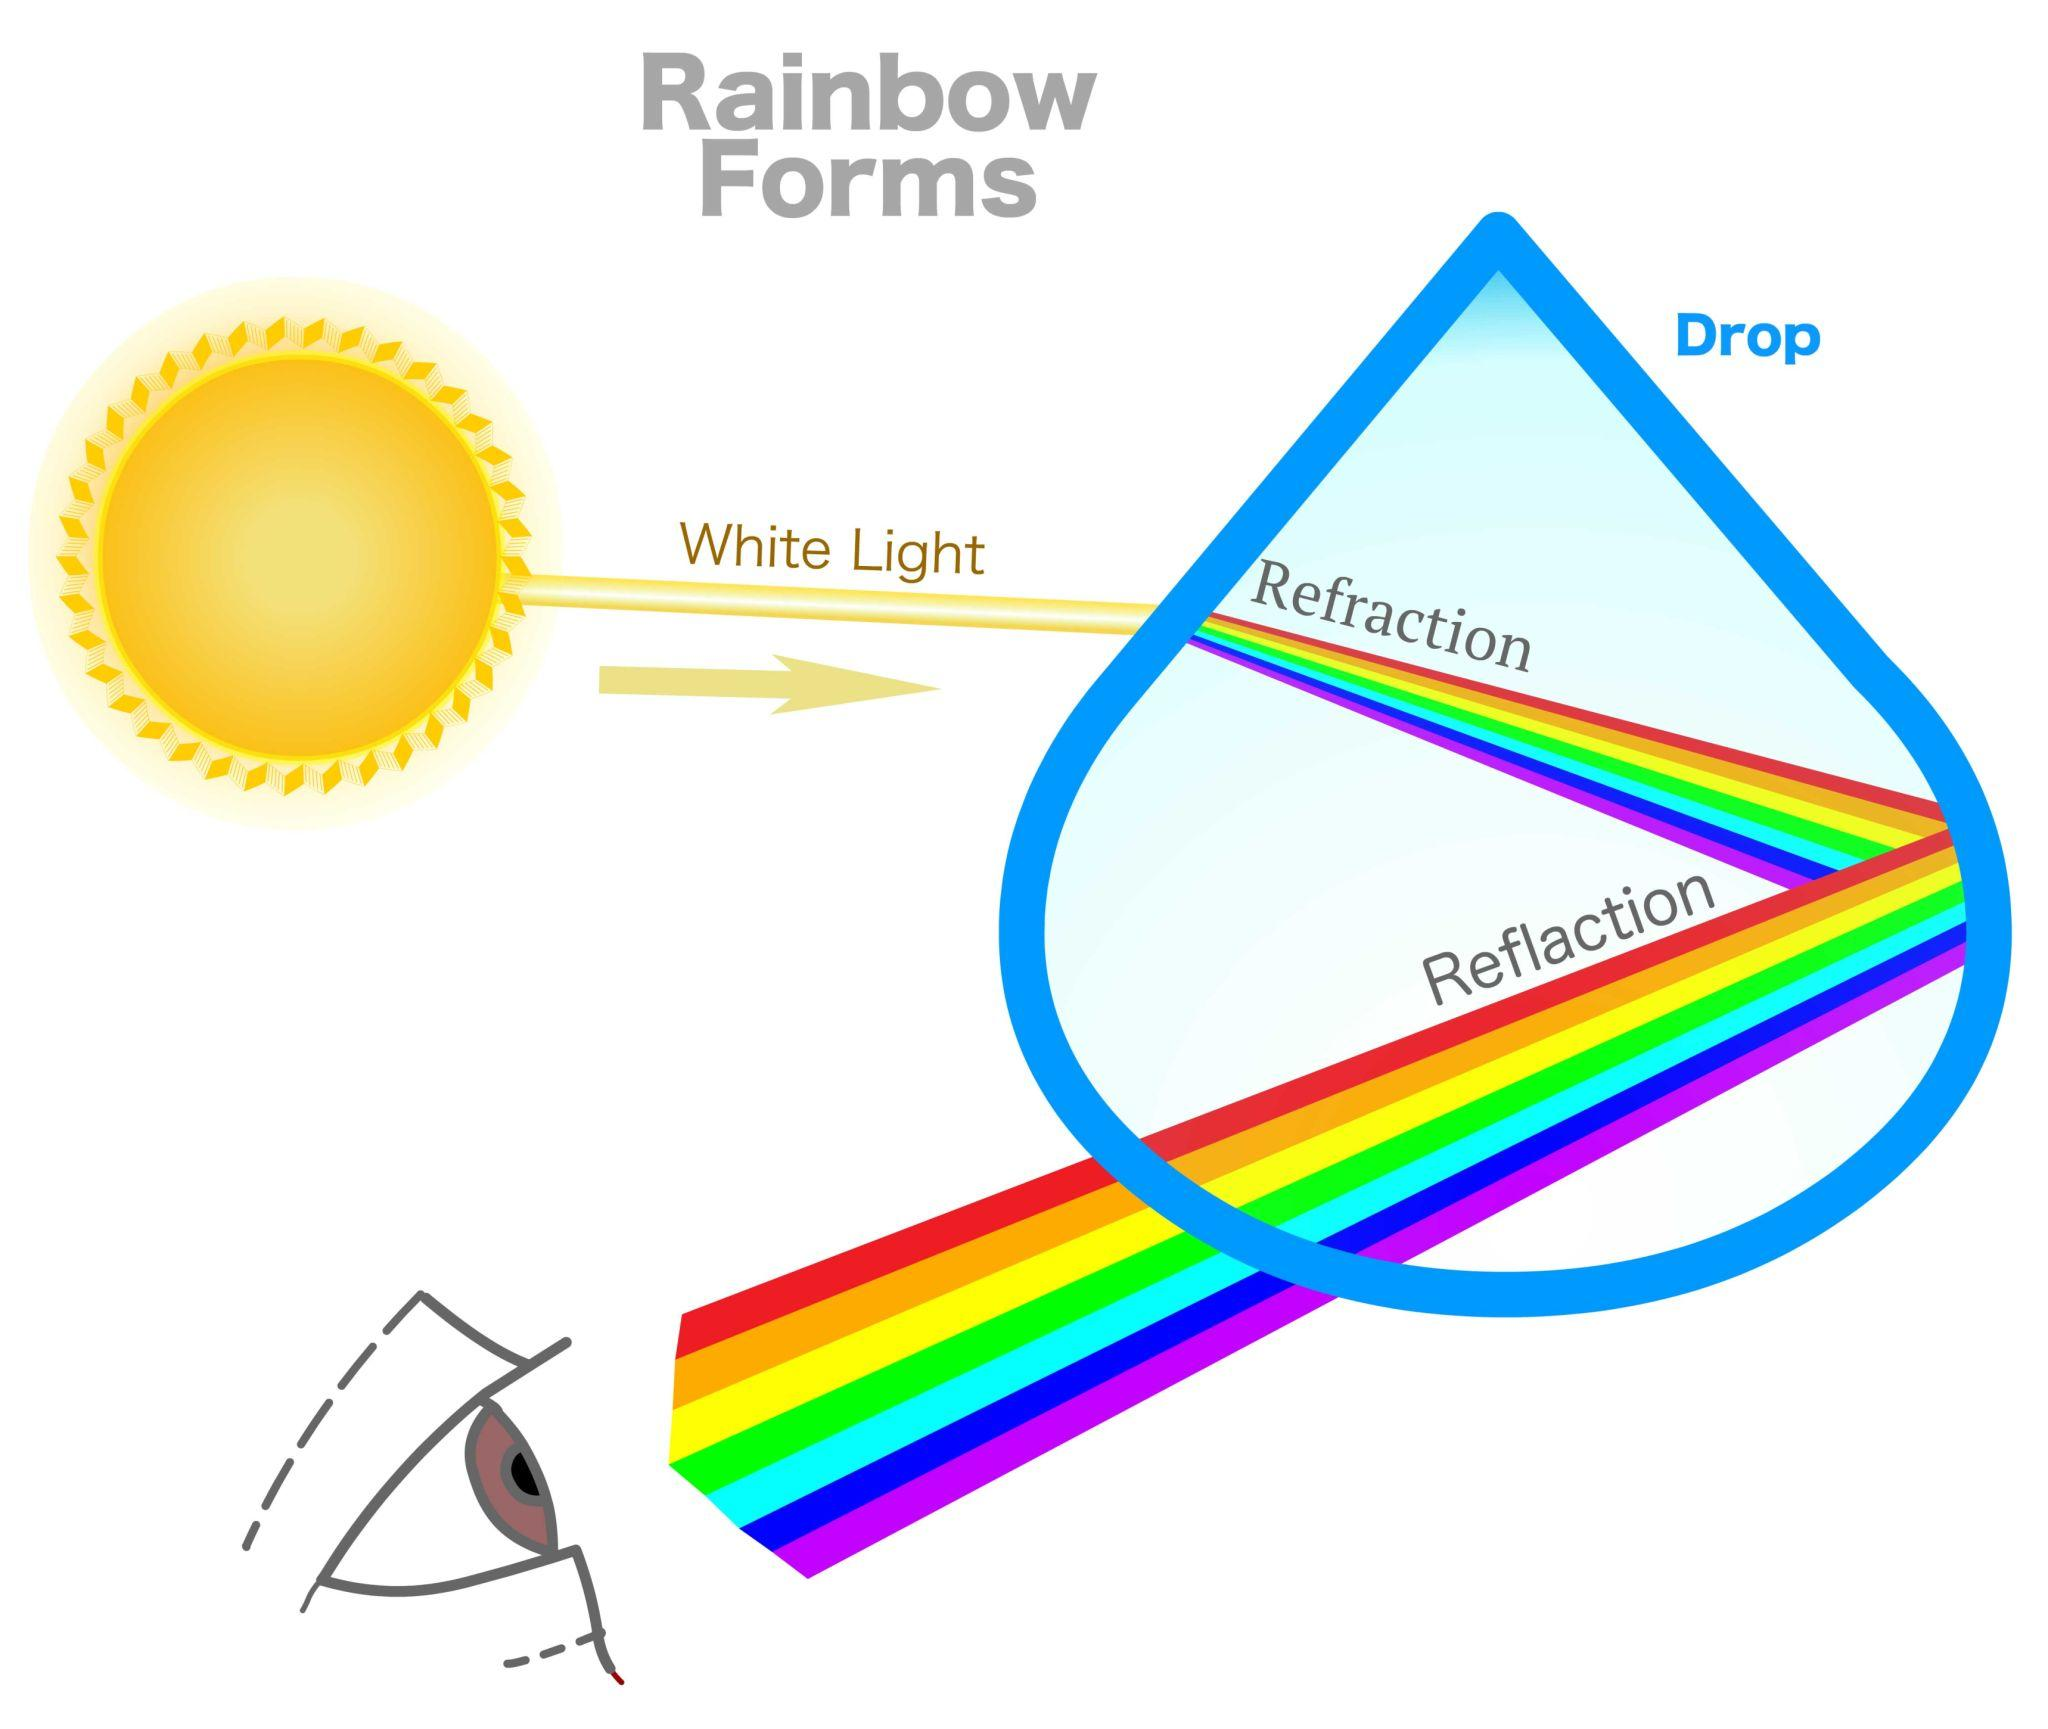
\includegraphics{../static/img/2026/rainbow1}}

רואים מה הולך כאן?! יש לנו טיפת גשם אחת שמפצלת את אור השמש לשלל צבעים
עליזים וכולם מגיעים לעין שלי. כל אחד מחלקי המשפט הזה נכון: באמת יש
טיפת גשם; היא באמת מפצלת את אור השמש לצבעים עליזים, ובאמת לעין שלי
מגיעים כל הצבעים הללו כשאני רואה גשם - \textbf{אבל הם לא מגיעים מאותה
טיפה}. זו הטעות הראשונה והגרועה ביותר שלי )ויש איורים חכמים יותר שנמנעים
מהפאשלה הזו ואביא כאלו בהמשך(. זה מה שתמיד שיגע אותי - אם אני חושב
על כל האור כאילו הוא מגיע אלי מנקודה אחת כשהוא מפוצל, אז למה האשליה
שנוצרת אצלי בראש היא שהוא מגיע מאיזור גדול במרחב? התשובה לזה פשוטה
- הוא לא. זה לא מה שקורה כאן. האיורים כמו זה למעלה קצת מטעים. הקשת
שאני רואה היא התוצאה של הרבה יותר טיפות שפועלות בו זמנית. כולן מפצלות
את האור לצבעים שונים, אבל האדום שאני רואה בקשת מגיע מטיפה אחת והכחול
מגיע מטיפה אחרת שנמצאת במקום שונה.

אוקיי, בואו ננסה להבין מה בעצם קורה כאן.

\section{מה זה אור?}

קשת בענן זו תופעה שמתרחשת משילוב של שלושה דברים:
\begin{enumerate}
\item השמש פולטת קרני אור שמגיעות לכדור הארץ.
\item קרני האור הללו עוברות דרך איזור באוויר שמלא בטיפות מים.
\item התוצאה של המפגש הזה של קרני האור והמים מגיעה אל העיניים שלנו.
\end{enumerate}
כלומר, כדי להבין עד הסוף מה גורם לקשת צריך לעקוב אחרי קרני אור במהלך
מסע מפותל שכולל יציאה מהשמש, התנגשות עם מים ואז התנגשות עם הפרצוף
שלי.

השלב הראשון במסע די פשוט: יש בשמש איזו מהומה שמערבת היתוך גרעיני ואקשן,
וכל זה לא רלוונטי לסיפור הזה בכלל. כתוצאה מהמהומה הזו נפלטות קרני
שמש לכל כיוון אפשרי. \textquotedblleft קרן שמש\textquotedblright{}
היא בעצם שם לקרינה אלקטרומגנטית, שהיא משהו שנע במהירות האור, ובנוסף
לכך יש לו \textbf{אורך גל}. יש הרבה סוגי קרינה אלקטרומגנטית שנבדלים
באורך הגל שלהם. למשל, יש \textbf{גלי רדיו}, שהאורך שלהם הוא החל מ-{\beginL 1\endL}
מילימטר, או בכתיב מתמטי \L{$10^{-3}$} מטר. הם כוללים את הגלים שמשתמשים
בהם לשידורי רדיו, לחימום במיקרוגל, למכ\textquotedblright מים וכדומה.
אנחנו נעזרים בגלים הללו כל הזמן אבל אנחנו לא רואים אותם והם גם לא
מפריעים לנו במיוחד באופן כללי.

בצד השני של הסקלה יש את הגלים הקצרים במיוחד: קרינת גמא, עם אורך גל
של בערך \L{$10^{-11}$} מטר וקצר יותר, וקרינת רנטגן שהיא בערך בין
\L{$10^{-8}$} ל-\L{$10^{-11}$}. זו קרינה הרבה יותר מסוכנת לנו מאשר
קרינת רדיו, כי ככל שאורך הגל של קרינה קצר יותר, כך היא יותר אנרגטית
)יש משהו שנקרא \textbf{תדירות} שהוא הפוך לאורך הגל - ככל שאורך הגל
גדל, התדירות קטנה, וככל שהתדירות גדולה יותר הקרינה אנרגטית יותר(.
כשקרינה מאוד אנרגטית מגיעה אלינו לגוף היא יכולה לעשות מהומות בתאי
הגוף שקרינה פחות עוצמתית לא יכולה לחולל אפילו אם יש הרבה ממנה. גם
זה לא סיפור שרלוונטי לנו הפעם אם כי הוא מאוד מעניין בפני עצמו. למרבה
המזל, השמש לא מוציאה הרבה קרינה כזו ומה שכן יוצא נבלע ברובו באטמוספירה.
מה שעדיין חודר ומגיע אלינו ומסכן אותנו ואנחנו מתמרחים נגד השמש בגללו
נקרא \textbf{קרינה אולטרה סגולה}, והיא נעה על הטווח שבין \L{$4\cdot10^{-7}$}
ו-\L{$10^{-8}$} מטר. חוץ ממנה, אם הולכים לצד השני של הסקלה, יש גם
קרינה עם אורך גל קצר יותר מקרינת רדיו שאנחנו עדיין לא יכולים לראות
- הקרינה \textbf{האינפרה אדומה} שעל הסקלה בין \L{$7\cdot10^{-7}$}
ועד \L{$10^{-3}$}. זה משאיר רק איזור אחד בסקלה שלא דיברנו עליו -
הקרינה שבין \L{$4\cdot10^{-7}$} ועד \L{$7\cdot10^{-7}$}. מסיבות
של המהומה שיש בתוך השמש ואקשן שציינתי, חלק נכבד מאוד מהקרינה של השמש
נמצא בתחום הצר הזה, ולכן אנחנו, שהתפתחנו בכוכב לכת שמקבל קרינה מהשמש
הספציפית הזו, היה משתלם לפתח חיישנים שמותאמים לטווח הזה והם כל כך
טובים שהם מסוגלים לזהות הפרשי אורכי גל קצרים יחסית בתוך הטווח הזה.
זה מה שאנחנו קוראים לו \textbf{אור נראה} )כי \textbf{אנחנו}, בני האדם,
יודעים לראות אותו(. יכולת ההפרדה שלנו לא מושלמת, אבל אנחנו רגילים
לראות שישה \textquotedblleft צבעים\textquotedblright{} שונים בתוך הטווח
הזה. הנה הם, מסודרים מהקצר לארוך ביותר. כדי להימנע מלכתוב \L{$10^{-7}$}
כל הזמן, בואו נתרגל לדבר על \textbf{ננומטר}. ננומטר הוא \L{$10^{-9}$}
מטר, ולכן \L{$4\cdot10^{-7}=400\cdot10^{-9}$} הוא \textquotedblleft{\beginL 400\endL}
ננומטר\textquotedblright , אז זה מה שאשתמש בו.
\begin{itemize}
\item סגול: {\beginL 380-450\endL} ננומטר.
\item כחול: {\beginL 450-500\endL} ננומטר.
\item ירוק: {\beginL 500-565\endL} ננומטר.
\item צהוב: {\beginL 565-590\endL} ננומטר.
\item כתום: {\beginL 590-625\endL} ננומטר.
\item אדום: {\beginL 625-750\endL} ננומטר.
\end{itemize}
זו ספציפית טבלה שדי העתקתי מויקיפדיה; לא כל המקורות מסכימים בדיוק
איפה צבע אחד נגמר והשני מתחיל, או אפילו איפה כל הספקטרום מתחיל ונגמר.
העניין הוא שצבעי הקשת הם עניין תרבותי לא פחות מאשר מדעי; כשמציירים
איור של קשת, נהוג להשתמש ב\textbf{שבעה} צבעים נפרדים זה מזה. בואו
נשווה בין שתי תמונות של ויקיפדיה: אחת של קשת אמיתית )שצולמה בישראל!(
והשניה של הייצוג הסימבולי המקובל של קשת:

\L{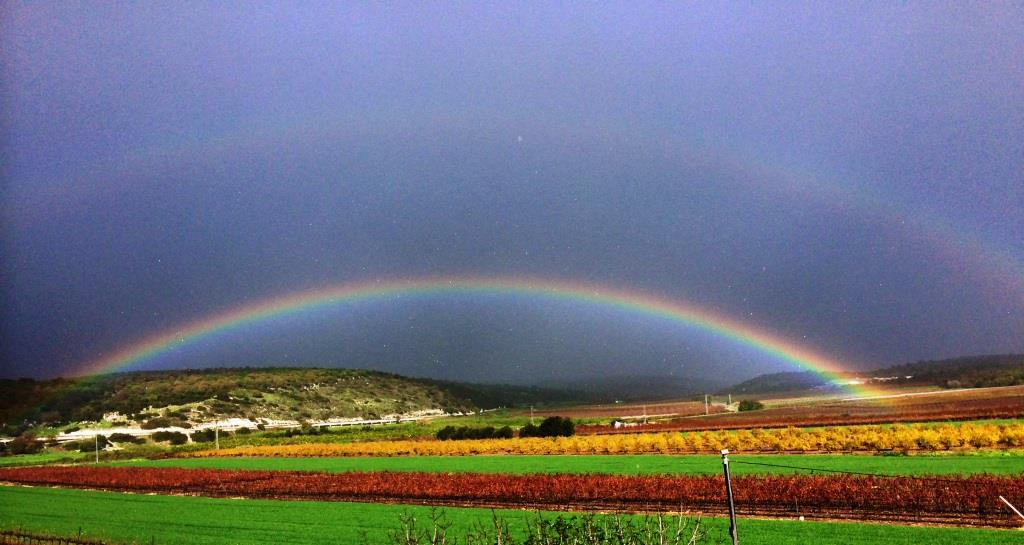
\includegraphics{../static/img/2026/rainbow2}}

\L{
\includegraphics{../static/img/2026/rainbow3}}

בייצוג הסימבולי רואים שבעה פסים נפרדים, כל אחד עם צבע שונה לגמרי.
זה כמובן לא מה שקורה במציאות - קשת אמיתית היא אור רציף שמשנה את אורך
הגל שאנחנו רואים בצורה רציפה ולא ברור מתי משהו מתחיל ונגמר וכמה צבעים
יש )ובתמונה רואים \textbf{עוד קשת} מעל הראשונה - מה זה?! כלומר, זה
משהו סטנדרטי שנקרא \textquotedblleft קשת כפולה\textquotedblright ,
זה לא מפתיע, אבל גם אותו אני לא באמת מבין - אבל עוד נבין במסגרת הפוסט
הזה(.

הייצוג הסימבולי קורא לצבע הפנימי ביותר \textquotedblleft סגול\textquotedblright{}
)\L{violet}(. אחריו מגיע \textquotedblleft כחול עמוק שנראה לנו טיפה
סגול\textquotedblright{} או בקיצור, \textbf{אינדיגו}. אחר כך מגיע \textquotedblleft כחול
בהיר שנראה לנו כמו תכלת\textquotedblright{} או בקיצור - \textbf{כחול}
)הסיפור מאחורי \textquotedblleft תכלת\textquotedblright , צבע שלא
קיים בחלק מהשפות, הוא מעניין בפני עצמו ולא ניכנס אליו(. אחר כך העניינים
הופכים לסטנדרטים יותר עם ירוק, צהוב, כתום ואדום. יש גם צבעים שהשתרשו
בשפה שלנו למרות שהם לא מופיעים בתוך הקשת - צבעים שמתקבלים רק משילוב
של צבעי בסיס כמו ורוד, חום, לבן, ארגמן, אפור וכו'. וכמובן, יש את השחור
שהוא היעדר צבע. כל אלו מעניינים מאוד אבל גם הם לא יהיו רלוונטיים לנו
כאן.

מה שחשוב לענייננו הוא שכאשר קרניים יוצאות מהשמש, הן מורכבות מקרינה
מכל הספקטרום. יש אור סגול ואינדיגו וכחול וירוק וצהוב וכתום ואדום,
כולם ביחד, באותו כיוון ממש. אל תחשבו עליהם בתור קרן שמש אחת אלא בתור
הרבה קרניים שונות שצמודות אחת לשניה וזזות באותו כיוון. איזה כיוון
זה? מהשמש אור נפלט לכל כיוון, מה שמסביר את האיור הזה ש-\L{ChatGPT}
יצר לי:

\L{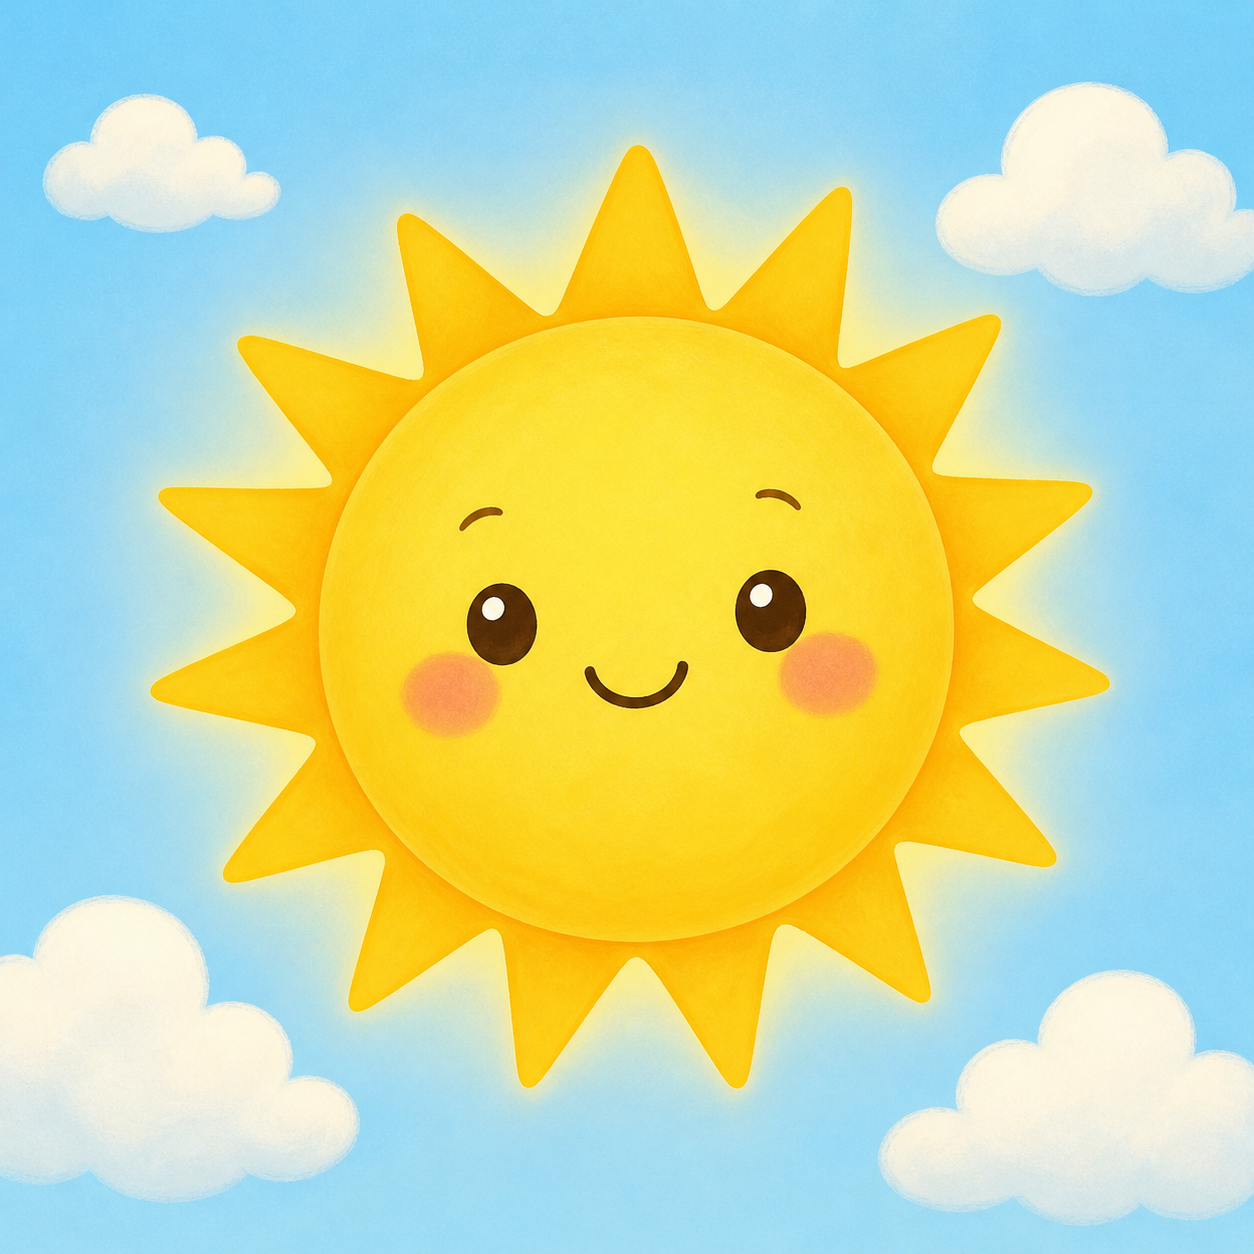
\includegraphics{../static/img/2026/rainbow4}}

אוהבים לצייר את השמש כשהיא מוקפת מכל כיוון בקרניים שיוצאות ממנה, או
צורה של שיניים, וכדומה. זה באמת מה שקורה. השמש \textbf{באמת} מוציאה
קרניים לכל כיוון אפשרי, אבל מה שאנחנו בכדור הארץ מקבלים הוא רק חלק
זעום מהקרניים שלה, ובגלל שהשמש כל כך רחוקה מאיתנו אפשר לחשוב על כל
הקרניים מהשמש שמגיעות אלינו כאילו הן מגיעות \textbf{מאותו כיוון בדיוק},
כלומר הן כולן קרניים מקבילות. כאילו השמש ירתה עלינו קרן לייזר. זה
חשוב, כי כשעוד מעט נדבר על מה קורה כשקרני השמש פוגשות טיפות מים, העניין
הקריטי ביותר בכל הסיפור יהיה איך שכל הקרניים באות במקביל.

גם הדבר הזה \textbf{מנוגד לאינטואיציה שלי}. למה? בגלל עוד תופעה יפה
שמערבת את קרני השמש - מה שקורה כשהשמש חודרת דרך עננים ומתקבל מה שנקרא
\L{Crepuscular rays} )\textquotedblleft קרני דמדומים\textquotedblright ?
אני לא מכיר תרגום לעברית עם שימוש נפוץ(, מה שנראה ככה בתמונה שלקחתי
מויקיפדיה:

\L{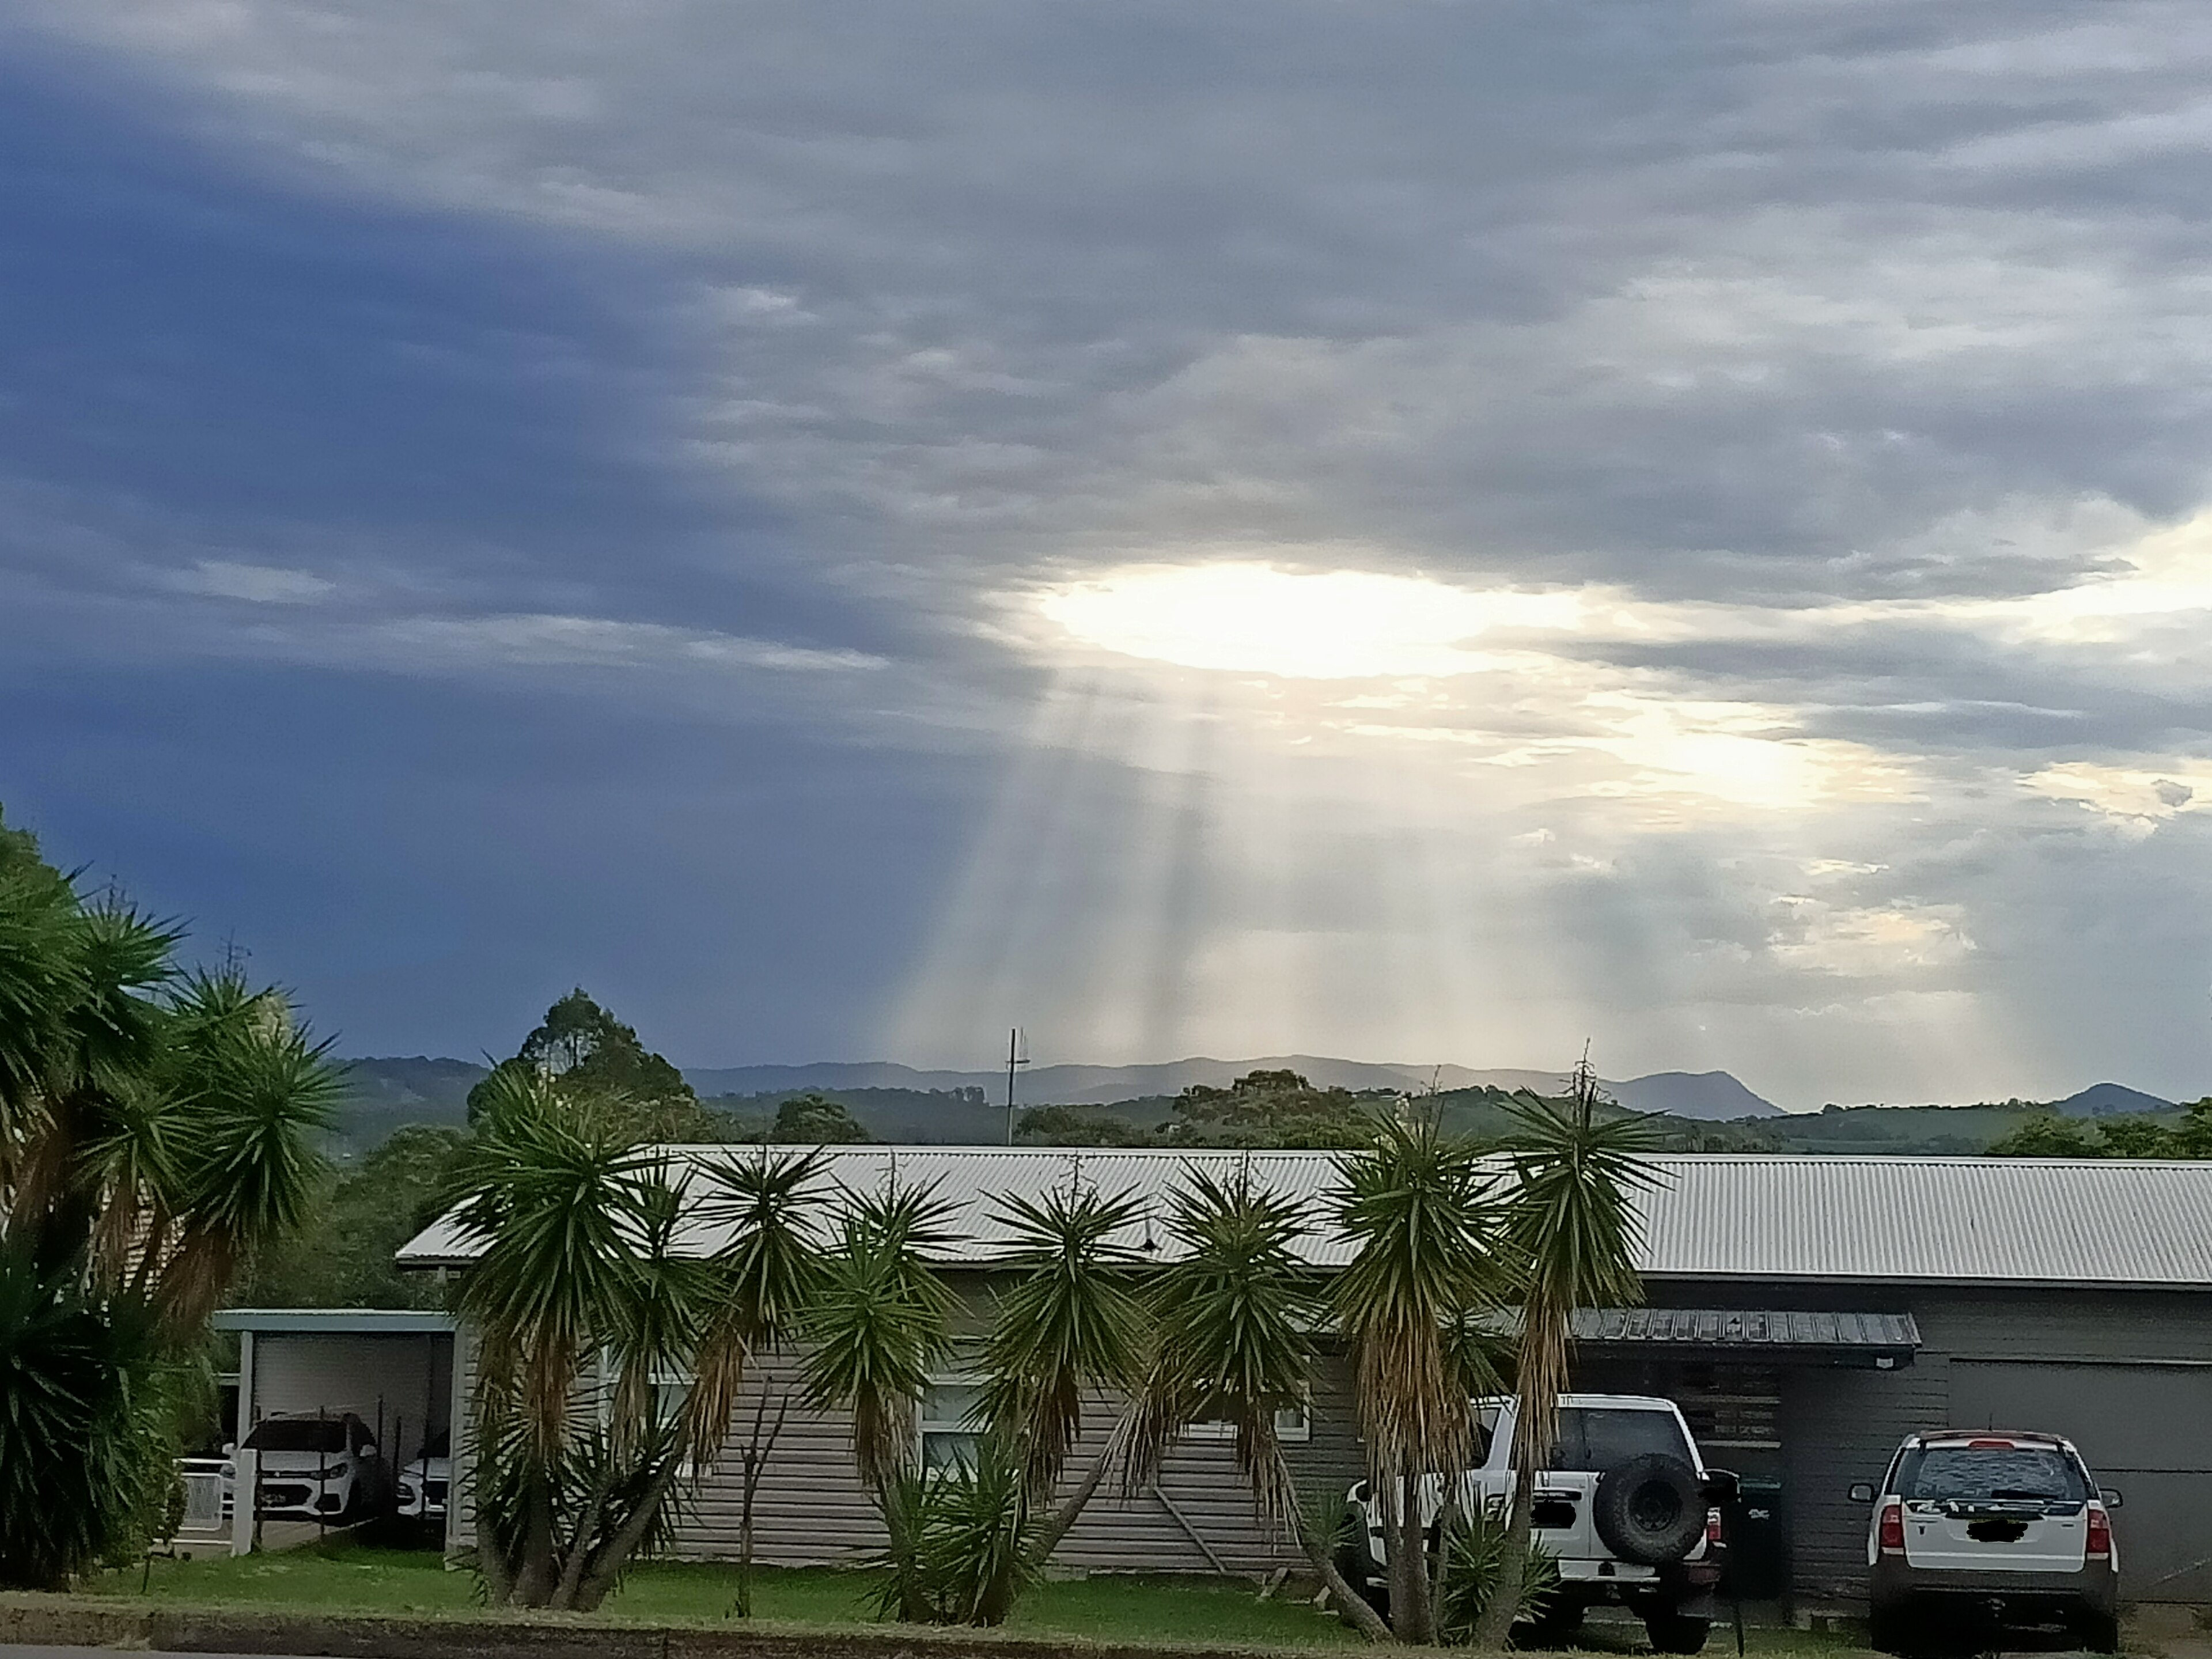
\includegraphics{../static/img/2026/rainbow5}}

בתמונה הזו נראה שהקרניים בוקעות משמש שנמצאת בדיוק מעל שכבת העננים
וכמו מנורה כזו יורה קרניים לכל כיוון אפשרי. בפועל אלו קרניים מקבילות
שנראות כאילו הן מגיעות ממקור משותף בגלל הפרספקטיבה שלנו - כמו פסי
הרכבת המקבילים שנראה שנפגשים באינסוף שהזכרתי לא מזמן \href{https://gadial.net/2026/04/05/dobble_and_projective_planes/}{בפוסט שלי}
על גאומטריה פרוייקטיבית )וחוץ מזה יש גם הסברים שטוענים שחלק מהקרניים
פשוט מתפזרות עקב החומרים שהן מתנגשות איתם באטמוספירה, בדומה לפיזור
שעוד מעט נדבר עליו שגורם ליצירת קשת(. בגלל אשליית \textquotedblleft השמש
ממש קרובה\textquotedblright{} שהקרניים הללו יוצרות הן חביבות על חלק
מהאנשים שמנסים לטעון שכדור הארץ שטוח - זה דיון מעניין בפני עצמו שלא
אכנס אליו - השורה התחתונה שצריך לצאת איתה מהסיפור היא שהאינטואיציה
שלנו שקרני האור הולכות לכל כיוון היא שגויה. כל הקרניים שמגיעות מהשמש
מגיעות במקביל זו לזו.

זה מסיים את הדיון שלנו על שלב {\beginL 1\endL}. אנחנו עכשיו יודעים
\textbf{מה} מגיע אלינו, ו\textbf{איך} )באיזה כיוון( הוא מגיע אלינו.
עכשיו נשאלת השאלה מה קורה כשהמשהו הזה מתנגש בטיפת מים.

\section{מה זה גשם}

בואו נחזור לרגע אל האיור ש-\L{ChatGPT} יצר לי ברוב טובו:

\L{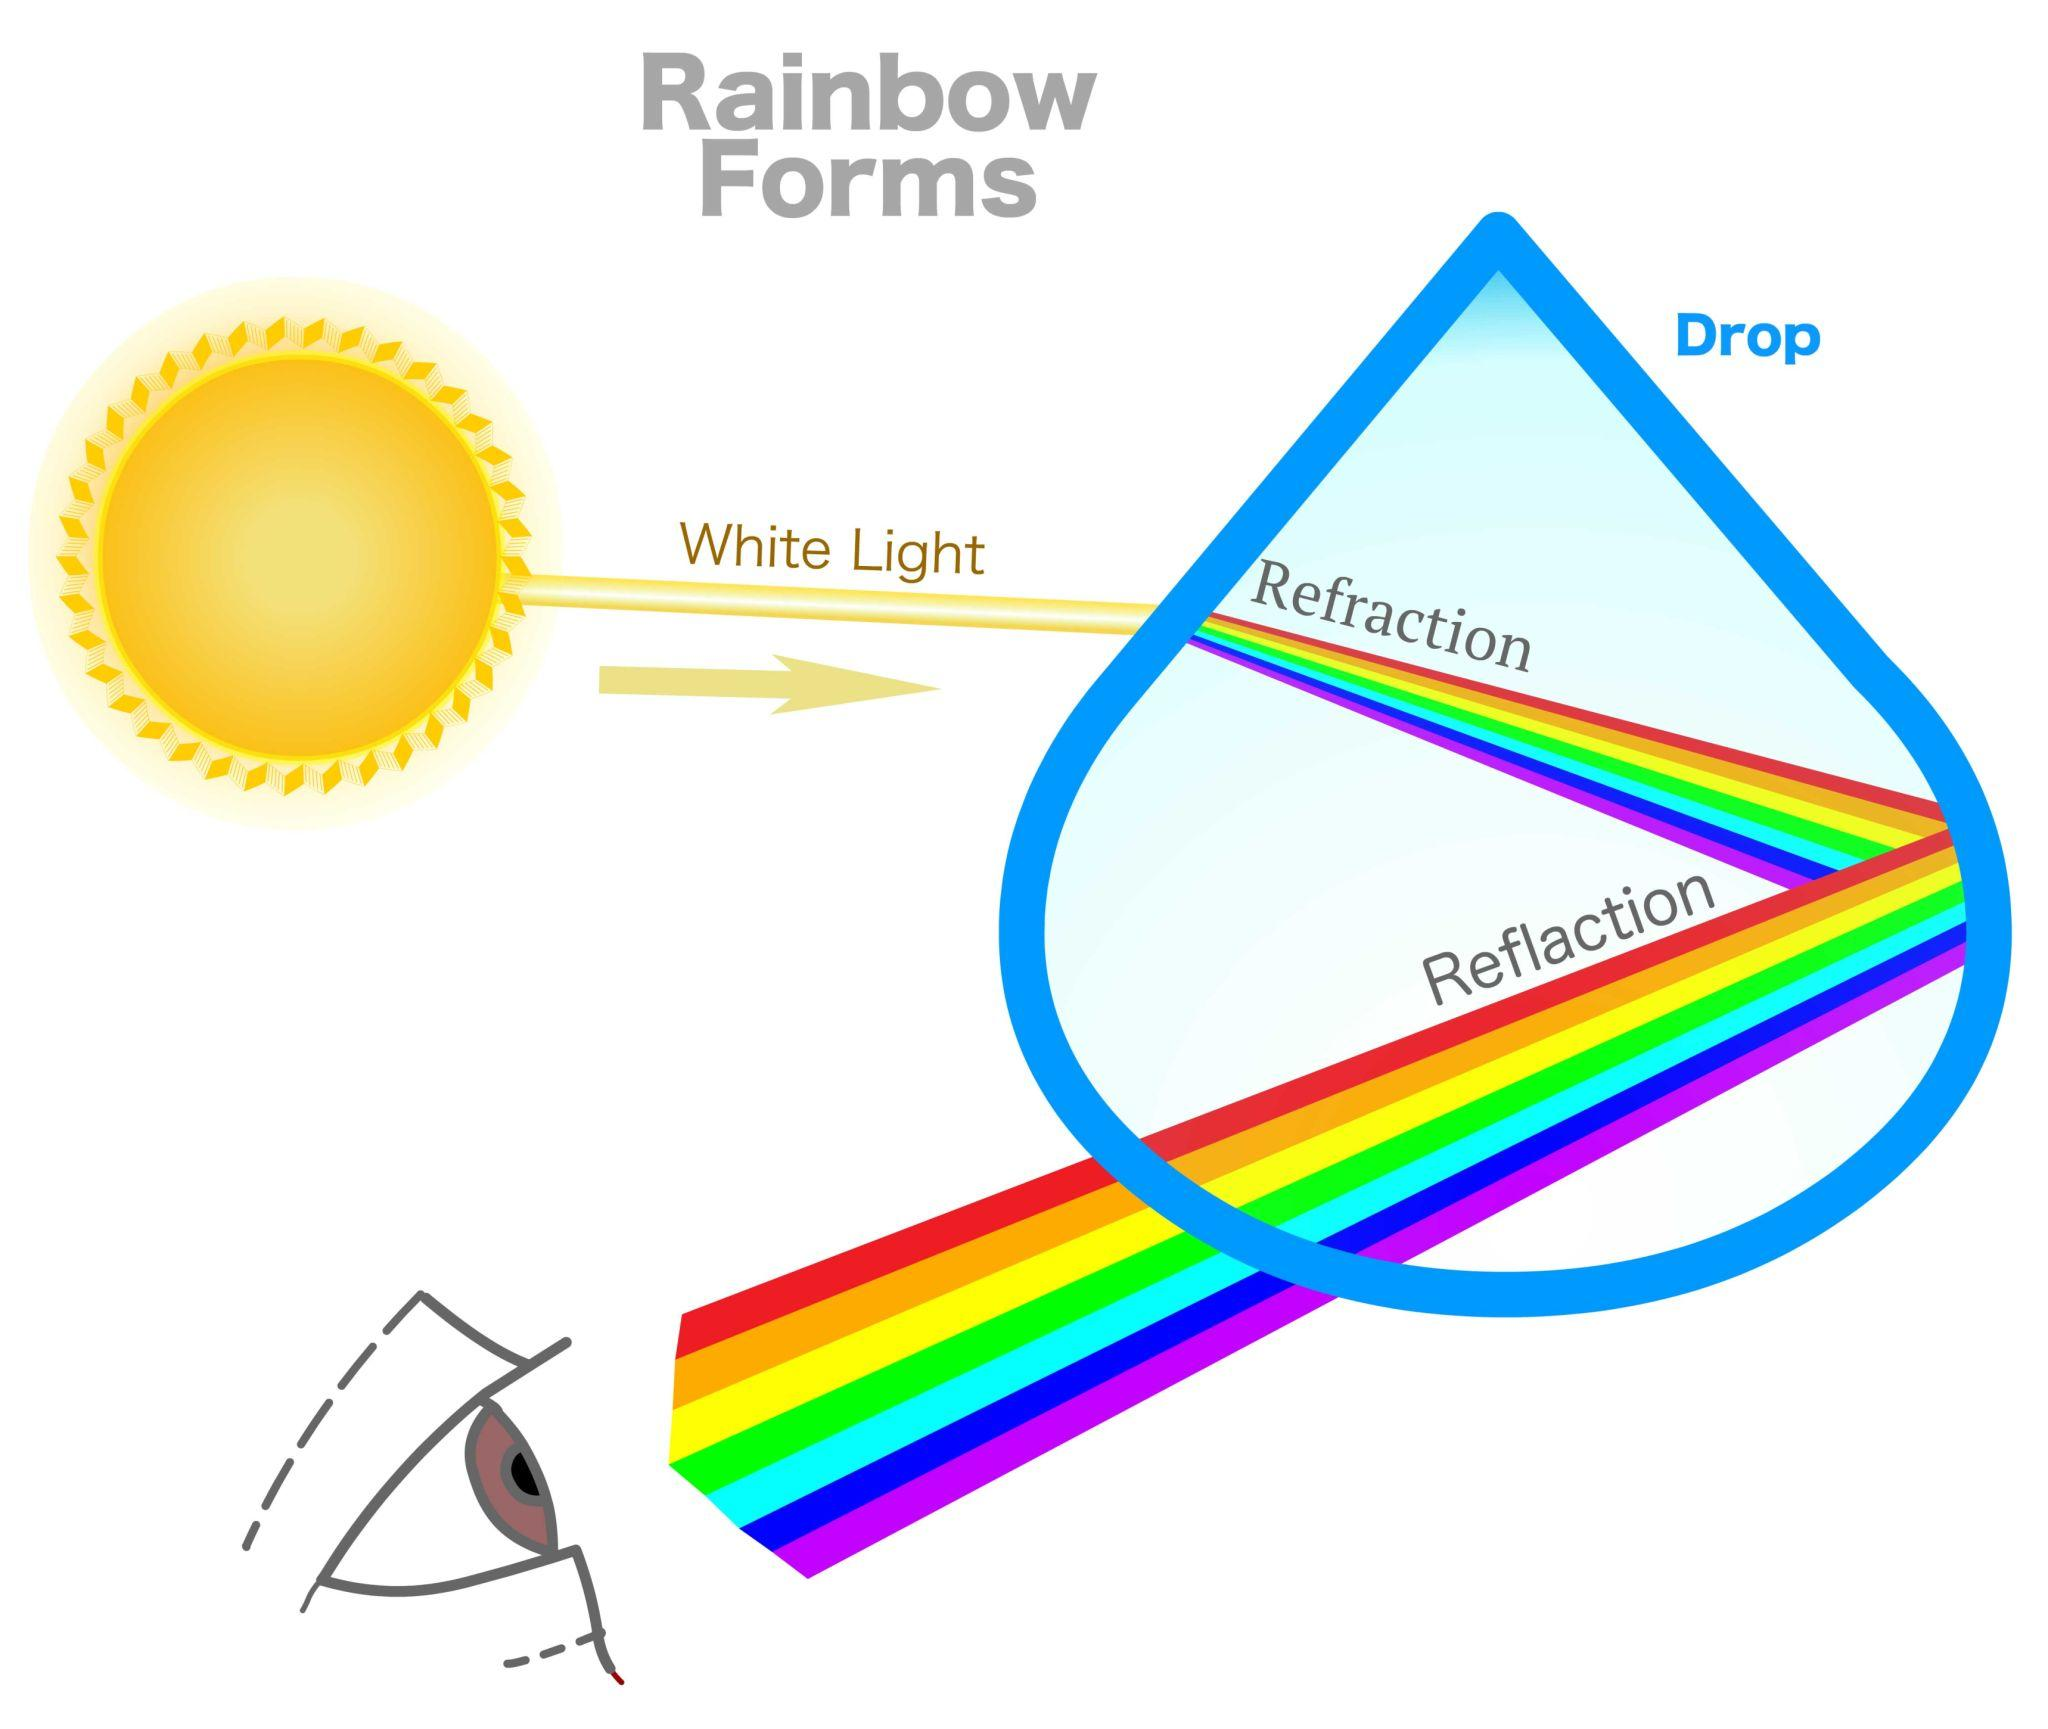
\includegraphics{../static/img/2026/rainbow1}}

כבר התלוננתי על דרך אחת שבה האיור הזה מטעה, אבל יש עוד דרך: \textbf{הצורה
של טיפת הגשם שגויה לחלוטין}. זו לא אשמת \L{ChatGPT} המסכן; האינטרנט
מלא באיורים מהז'אנר הזה שבהם טיפת הגשם נראית ככה. אבל טיפות גשם לא
נראות ככה. בכלל. אף פעם. למרות שאם תבצעו חיפוש זריז על \L{raindrop}
תמצאו אינספור איורים שנראים בדיוק ככה. למה? למה שנחשוב שככה נראות
טיפות גשם? ובכן, אולי כי זו הצורה הנפוצה שבה \textbf{אנחנו }רואים
טיפות מים במציאות. למשל, כשיש ברז מטפטף אנחנו רואים מים מצטברים ויוצרים
טיפה שנראית בדיוק ככה - \textbf{עד שהיא נופלת}. או כשיש גשם ומים נופלים
לנו על החלון הם מצטברים למשהו שנראה ככה, וכן הלאה. אבל טיפת גשם שנופלת?
היא לא נראית ככה. אם היא קטנה מספיק, היא תיראה כמו כדור מושלם או קרוב
לכך, ואם היא כבדה יותר היא תהיה פחוסה עם מעין בליטה בתחתית שלה בגלל
ההתנגדות של האוויר. הניתוח שלי של \textquotedblleft מה קורה כשאור
מתנגש בטיפת גשם\textquotedblright{} יניח שהטיפה היא כדור מושלם - ובאמת
ככל שהטיפה מאבדת מהשלמות הזו הניתוח שאציג פחות טוב ולכן קשת שנוצרת
מגשם חזק היא יותר מצ'וקמקת.

אז מה יש לנו? משהו שנראה ככה:

\L{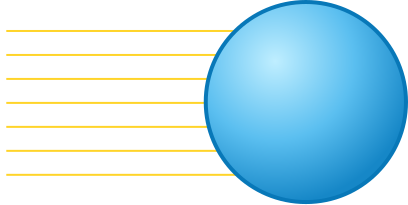
\includegraphics{../static/img/2026/rainbow_drop_stage1}}

הקווים הצהובים האופקיים הם קרני האור. הדיון הארוך שניהלתי קודם הסביר
למה הן כולן מקבילות, אבל למה בעצם כולן \textbf{אופקיות}, כלומר מגיעות
בקו ישר ולא בזווית? ובכן, במציאות הן לא, וזה דווקא יהיה חשוב ונדבר
על זה, אבל גם אם הקרניים היו מגיעות בזווית אחרת, אפשר היה פשוט לסובב
את התמונה ולקבל את אותו הדבר. לצורך הניתוח של מה קורה לקרן כשהיא פוגעת
בטיפה אפשר לדמיין שכולן מאוזנות; אחר כך, כשנסתכל על הסיפור ברמת המקרו
נכניס גם את הזווית שלהן לתמונה.

עכשיו, מה מבדיל קרניים שונות בתמונה זו מזו? \textbf{הגובה} שלהן. אם
נדמיין שעובר קו אופקי של ציר באמצע הטיפה, אז אפשר להבדיל בין כל קרן
אור על פי הגובה שלה מעלה/מתחת לציר הזה. בעצם למה לדמיין כשאפשר לצייר:

\L{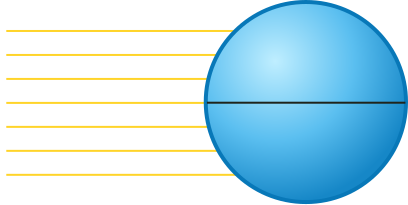
\includegraphics{../static/img/2026/rainbow_drop_stage2}}

הגובה של הקרן משפיע באופן דרסטי על מה שיקרה לה בתוך הטיפה. בגדול,
כל קרן שנכנסת לטיפה חווה שלושה דברים:
\begin{enumerate}
\item במהלך \textbf{הכניסה} לטיפה, חלק מהקרן מוקפץ החוצה - מה שנקרא \textbf{החזרה}
של האור.
\item \textbf{אחרי} הכניסה לטיפה, האור שנכנס \textbf{משנה כיוון}, מה שנקרא
\textbf{שבירה} של האור.
\item במהלך \textbf{היציאה} מהטיפה, חלק מהקרן שוב הולך להיות מוקפץ חזרה,
ויתר הקרן תצא החוצה.
\end{enumerate}
כלומר )אם מתעלמים מהאור שנבלע בתוך הטיפה ובכל מקרה לא מעניין אותנו(,
אותה הקרן התפצלה תוך כדי האינטראקציה שלה עם הטיפה לשלושה קרניים שונות:
\begin{enumerate}
\item הקרן שעברה את כל המהומה הזו ויצאה מהצד השני: היא לא הולכת לעניין אותנו
בכלל. כמו שנראה בהמשך, אנחנו בכלל לא רואים אותה כשרואים קשת.
\item הקרן שחזרה בהתחלה: אנחנו הולכים לראות את הקרניים הללו, אבל הן לא ייראו
לנו כמו קשת אלא כמו אור רגיל, כמו מה שאנחנו רואים כל הזמן שמוחזר מכל
דבר בערך. אז גם זה לא יהיה רלוונטי לנו.
\item הקרן שנשברה \textbf{ואז גם} הוחזרה: כאן מתרחש האקשן. הקרן הזו הולכת
להתפצל לשלל קרניים שנעות בכיוונים קצת שונים בהתאם לצבע של הקרן, וזה
מה שאנחנו הולכים לראות בתור קשת.
\end{enumerate}
אחת המיסקונספציות הבסיסיות שלי לגבי קשת בענן הייתה שהאקשן הוא דווקא
עם קרן {\beginL 1\endL}, זו שנכנסת ויוצאת מהצד השני. זה כמובן לא נכון.
קרן כזו לא תתפצל לצבעים שונים ולכן כל הסיפור לא רלוונטי לגביה. הסיבה
לקשת היא השילוב בין שתי תופעות שונות שקרן מס' {\beginL 3\endL} עוברת:
גם \textbf{שבירה} וגם \textbf{החזרה}. אז בואו נבין מה התופעות הללו
אומרות - למרבה השמחה, מבחינה מתמטית הן פשוטות מאוד.

\section{על שבירה והחזרה}

שבירה והחזרה הם שני היבטים של אותו אירוע - קרן אור שעוברת מתווך אחד
לאחר. בואו נצייר את שתיהן ביחד:

\L{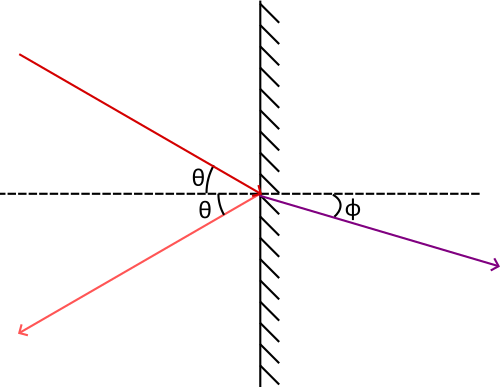
\includegraphics{../static/img/2026/reflection_refrection}}

מה שקורה באיור הזה הוא הדבר הבא. ראשית, יש לנו את הגבול בין שני התווכים
)למשל, התווך של האוויר והתווך של המים. אני מתאר את הגבול בזה בתור
קו אנכי עם מין קווים אלכסוניים קצרים שצמודים אליו ומסמלים במקרה הזה
\textquotedblleft כאן נגמר האוויר ומתחיל החומר האחר שדרכו האור עובר\textquotedblright .

שנית, הדרך הנוחה ביותר לתאר מה קורה לאור היא להסתכל על הקו \textbf{המאונך}
לגבול, מה שבאיור הוא הקו המקווקו. זה נקרא \textbf{הנורמל} למשטח. עכשיו,
את הקרן המקורית אני מתאר בעזרת הקו האלכסוני משמאל-למעלה, ואני מסמן
את הזווית בינו ובין הנורמל ב-\L{$\theta$}. אחרי הפגיעה בקו הגבול,
הקרן מתפצלת לשתיים: הקרן ש\textbf{מוחזרת} פונה למטה ושמאלה, והקרן
שנשברת פונה למטה וימינה. גם עבור שתיהן אני מסתכל מה הזווית שהן יוצרות
עם הנורמל. עבור ההחזרה, הזווית הזו פשוטה: זו בדיוק \L{$\theta$} המקורית!
עבור השבירה הסיפור יותר מסובך אז אני מסמן אותה בינתיים בתור \L{$\phi$}.

איך מוצאים את זוויות ההחזרה והשבירה? הסבר מתמטי אמיתי יצטרך להיכנס
לאופי הגלי של האור וזה פוסט מרתק בפני עצמו אבל ארוך מדי להפעם. במקום
זה אני הולך לדבר על משהו שנשמע כמו רמאות גמורה - \textbf{עקרון פרמה}.

מה זה עקרון פרמה? ובכן, אני אעתיק את מה שכתוב כרגע בויקיפדיה העברית:
\textquotedblleft עקרון פרמה או עקרון הזמן המינימלי קובע כי בתנועתה
בין שתי נקודות נתונות, עוברת קרן אור במסלול בו זמן תנועתה הוא הקצר
ביותר\textquotedblright . זה ניסוח טוב כי הוא תופס במדויק את הניסוח
ששמעתי בהמון מקומות של העקרון הזה - וזה בבירור \textbf{שגוי לגמרי}
כי תסתכלו שניה על האיור, המסלול שעוברת הקרן שמוחזרת הוא בוודאי לא
המסלול האופטימלי מנקודת ההתחלה לנקודת הסיום, היה אפשר פשוט ללכת בקו
ישר. אז כן, עקרון פרמה האמיתי קצת יותר מורכב; בהקשר שלנו מספיק יהיה
לדבר על \textquotedblleft הדרך האופטימלית בהינתן אילוצים\textquotedblright{}
כשהאילוץ עבור החזרה הוא שחייבים לגעת במשטח )הקו האנכי באיור( ואילו
עבור שבירה, וזה נחמד, לא נצטרך עוד אילוצים והעקרון יעבוד גם בניסוח
הפשוט שלו.

העקרון נשמע הזוי כי איך בדיוק קרן האור יודעת מי יהיה המסלול שבו זמן
תנועתה הוא הקצר ביותר, אבל זה מה שנחמד פה: אור הוא הרי לא באמת קרן,
הוא \textbf{גל}, ואם נכנסים לניתוח המתמטי של גלים, רואים שעקרון פרמה
באמת מתקבל וזה נראה פחות מפתיע כי גל הוא משהו שסוג של נמצא בכל המרחב,
אז הוא יכול \textquotedblleft לבדוק את כל האפשרויות בו זמנית\textquotedblright .
אבל כאמור, זה לפוסט אחר. בפוסט הזה אני ארצה להראות איך משתמשים בניסוח
הדי פשוט של עקרון פרמה כדי למצוא את זוויות השבירה וההחזרה. למי שאין
להם כוח למתמטיקה הזו אפשר לקפוץ לחלק הבא - כל מה שאנחנו באמת צריכים
להמשך הוא את הקטע של \textquotedblleft זווית ההחזרה שווה לזווית הפגיעה\textquotedblright{}
שכבר ראינו, ואת זה שזווית השבירה \L{$\varphi$} היא לא אבסולוטית,
אפילו לא עבור המקרה של \textquotedblleft מעבר מאוויר אל מים\textquotedblright ,
אלא תלויה באורך הגל של האור )ועל זה אדבר עוד מעט(.

מכיוון שאנחנו עוסקים בפיזיקה, יש כמובן שתי דרכים למצוא את זווית ההחזרה
בעזרת עקרון פרמה - דרך אחת שהיא פשוטה ויפהפיה ואלגנטית ומרגישה כמו
רמאות ודרך שניה טכנית אבל הפעם לא בצורה כואבת מדי. בואו נתחיל עם הדרך
הפשוטה. נניח שאנחנו נמצאים בנקודה \L{$A$} ומשגרים קרן אל מראה. היא
פוגעת בה בזווית \L{$\theta_{1}$}, קופצת חזרה ממנה בזווית\L{$\theta_{2}$}
ומגיעה לנקודה \L{$B$}. הנה הטריק: אנחנו יכולים להסתכל על \textbf{ההשתקפות
במראה} של הנקודה \L{$A$} ולסמן אותה \L{$A^{\prime}$}. המסלול שהקרן
האמיתית עושה מ-\L{$A$} אל המראה משתקף בתוך המראה, כך שנראה שיש קרן
שעושה מסלול מ-\L{$A^{\prime}$}אל \L{$B$}. ככה זה נראה:

\L{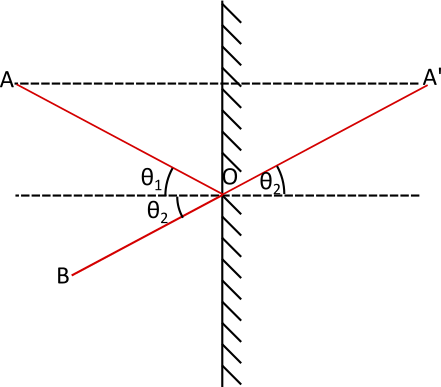
\includegraphics{../static/img/2026/reflection2}}

ה\textquotedblright רמאות\textquotedblright{} שאני עושה היא להחיל את
עקרון פרמה \textbf{על הנקודה הדמיונית בתוך המראה}. כלומר, אני אומר
שהקרן מהנקודה )הדמיונית( \L{$A^{\prime}$} אל \L{$B$} עוברת במסלול
המהיר ביותר בין שתי הנקודות הללו. מכיוון שהתנועה \textquotedblleft בתוך\textquotedblright{}
המראה היא באותה מהירות כמו התנועה \textquotedblleft מחוץ\textquotedblright{}
למראה, המסלול המהיר ביותר הוא גם הקצר ביותר )זאת להבדיל ממה שיקרה
עם שבירה ועוד מעט נראה(. המסלול הקצר ביותר בין שתי נקודות בגאומטריה
אוקלידית הוא הקו הישר ביניהן, ולכן הקרן שאנחנו רואים נמצאת על הקו
הישר \L{$A^{\prime}B$}. עכשיו, שימו לב ששתי הזוויות שסימנתי ב-\L{$\theta_{2}$}
הן מה שנקרא \textbf{זוויות קודקודיות} ולכן שוות זו לזו - זה עובד בזכות
העובדה ש-\L{$A^{\prime}B$} הוא קו ישר. מה שנשאר להשתכנע בו הוא ש-\L{$\theta_{1}=\theta_{2}$},
וזה נובע מכך שהמשולש \L{$AA^{\prime}O$} הוא \textbf{שווה שוקיים}
כי \L{$AO$} ו-\L{$A^{\prime}O$} הן השתקפויות זו של זו במראה )אם
לא מקבלים את זה כמובן מאליו אפשר גם יותר טרחני - אם נסמן את הנקודה
שבה הישר \L{$AA^{\prime}$} חותך את המראה ב-\L{$C$} נקבל שהמשולש
\L{$ACO$} חופף ל-\L{$A^{\prime}CO$} כי הם חולקים זווית ישרה ואת
הצלע \L{$CO$} ואילו הצלעות \L{$AC,A^{\prime}C$} שוות כי זו ממש ההגדרה
של כך ש-\L{$A^{\prime}$} היא ההשתקפות של \L{$A$}, כך שקיבלנו חפיפת
צלע-זווית-צלע שממנה נובע ש-\L{$AO=A^{\prime}O$}(, ועכשיו רק נשאר
להשתמש בכך שזוויות הבסיס של \L{$AA^{\prime}O$} הן \L{$\theta_{1},\theta_{2}$}
כי הן מה שנקרא \textbf{זוויות מתחלפות} בין ישרים מקבילים עם ה-\L{$\theta_{1},\theta_{2}$}
שלמטה.

אוקיי, אז זה הפשוט והאלגנטי, מה המסובך? במקרה המסובך אני לא מספר מעשיות
על נקודות \L{$A^{\prime}$} קסומות שבתוך המראה. אין כלום בתוך המראה.
ככה זה נראה:

\L{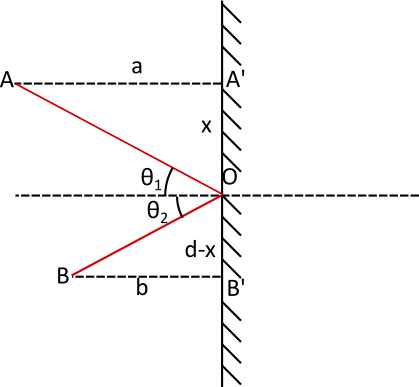
\includegraphics{../static/img/2026/reflection3}}

מה אני אומר פה: אוקיי, יש לנו נקודות \L{$A,B$} שרירותיות לגמרי מאותו
צד של המראה ואני שואל את השאלה \textquotedblleft מה המסלול שתעבור
קרן אור שיוצאת מ-\L{$A$}, פוגעת במראה ומגיעה אל \L{$B$}\textquotedblright .
עקרון פרמה )בניסוח התקין שלו( מבטיח לי שזה הולך להיות המסלול הקצר
ביותר מבין כל המסלולים שמתחילים ב-\L{$A$}, נגמרים ב-\L{$B$} \textbf{ופוגעים
במראה}. אז אני מסמן את הכל באותיות. ראשית, \L{$A^{\prime},B^{\prime}$}
הן ההטלות של הנקודות \L{$A,B$} על המראה ואילו \L{$a,b$} הם המרחקים
של הנקודות \L{$A,B$} מהמראה )כלומר האורכים של \L{$AA^{\prime}$}
ושל \L{$BB^{\prime}$}(. שנית, \L{$d$} הוא האורך של \L{$A^{\prime}B^{\prime}$}
- המרחק בין ההטלות של הנקודות הללו על המראה. כל הערכים הללו הם \textbf{קבועים}
שנתונים מראש בהגדרת הבעיה ולא תלויים במסלול זה או אחר.

עכשיו, אני מסמן ב-\L{$O$} נקודה \textbf{שרירותית} על המראה, כשהאילוץ
היחיד שלי עליה היא שהיא על \L{$A^{\prime}B^{\prime}$} )לא קשה לראות
שאם נקודת הפגיעה של הקרן מ-\L{$A$} אל \L{$B$} לא תהיה שם, הקרן תהיה
יותר ארוכה מכל קרן שכל פוגעת שם(. אני מסמן ב-\L{$x$} את האורך של
\L{$A^{\prime}O$} ולכן האורך של \L{$OB^{\prime}$} יהיה \L{$d-x$}.
עכשיו אני יכול לחשב את האורך הכולל של הקו האדום כפונקציה של \L{$x$}.
ראשית, \L{$AA^{\prime}O$} הוא משולש ישר זווית שאורכי האנכים שלו הם
\L{$a,x$} ולכן ממשפט פיתגורס האורך של \L{$AO$} הוא \L{$\sqrt{x^{2}+a^{2}}$},
ובאופן דומה האורך של \L{$OB$} הוא \L{$\sqrt{\left(d-x\right)^{2}+b^{2}}$}.
לכן הפונקציה שנותנת לי את האורך הכולל של הקרן מ-\L{$A$} אל \L{$B$}
היא

\L{$L\left(x\right)=\sqrt{x^{2}+a^{2}}+\sqrt{x^{2}-2dx+d^{2}+b^{2}}$}

המטרה שלי היא למצוא את \L{$x$} שעבורו \L{$L\left(x\right)$} מינימלית.
זו \href{https://gadial.net/2011/01/15/derivative_and_extremal_problems_1/}{בעיית קיצון בסיסית}
בחדו\textquotedblright א; הדרך לפתור אותה היא לגזור את \L{$L\left(x\right)$},
למצוא \L{$x_{0}$} כך ש-\L{$L^{\prime}\left(x_{0}\right)=0$}, ולוודא
ש-\L{$L^{\prime\prime}\left(x_{0}\right)>0$} כך שזו נקודת מינימום.
לגזור דברים עם שורשים זה \textbf{כואב}, אבל מצד שני \textbf{זה לא
כואב} כי אנחנו יודעים בדיוק איך עושים את זה, לא צריך להיות יצירתיים
או משהו. הנה, אני עושה את זה. הטריק הוא לכתוב

\L{$L\left(x\right)=\left(x^{2}+a^{2}\right)^{\frac{1}{2}}+\left(x^{2}-2dx+d^{2}+b^{2}\right)^{\frac{1}{2}}$}

ואז לגזור את זה כמו שגוזרים פולינום, כלומר על פי הכלל \L{$\left(x^{n}\right)^{\prime}=nx^{n-1}$},
רק שהפעם עם \L{$n=\frac{1}{2}$} )זה עדיין עובד(. בגלל שבתוך הסוגריים
יש משהו יותר מורכב מסתם \L{$x$}, צריך להשתמש \textbf{בכלל השרשרת},
\L{$f\left(g\left(x\right)\right)^{\prime}=f^{\prime}\left(g\left(x\right)\right)\cdot g^{\prime}\left(x\right)$},
כלומר אני צריך לקחת את מה שבתוך הסוגריים, לגזור גם אותו, ולכפול בזה.
גזירה פנימית כזו של הסוגריים השמאליים תיתן לי \L{$2x$} ושל הסוגריים
הימניים תיתן לי \L{$2x-2d$} ולכן בסך הכל נקבל

\L{$L^{\prime}\left(x\right)=\frac{1}{2}\left(x^{2}+a^{2}\right)^{-\frac{1}{2}}\cdot2x+\frac{1}{2}\left(x^{2}-2dx+d^{2}+b^{2}\right)^{-\frac{1}{2}}\left(2x-2d\right)$}

\L{$=\frac{x}{\sqrt{x^{2}+a^{2}}}+\frac{x-d}{\sqrt{\left(d-x\right)^{2}+b^{2}}}$}

לא כזה נורא! את זה אני צריך להשוות לאפס ולכן אחרי העברת אגפים אני
אקבל

\L{$\frac{x}{\sqrt{x^{2}+a^{2}}}=\frac{d-x}{\sqrt{\left(d-x\right)^{2}+b^{2}}}$}

אבל שימו לב מה קורה פה - עכשיו יש לי ממש אורכים של צלעות של המשולשים
המקוריים בביטוי הזה. קיבלתי

\L{$\frac{\left|A^{\prime}O\right|}{\left|AO\right|}=\frac{\left|B^{\prime}O\right|}{\left|BO\right|}$}

עכשיו, הזווית \L{$A^{\prime}AO$} היא \L{$\theta_{1}$}, שוב בגלל
נימוקי זוויות מתחלפות, והביטוי \L{$\frac{\left|A^{\prime}O\right|}{\left|AO\right|}$}
הוא על פי הגדרה סינוס של הזווית הזו, ובאופן דומה גם עבור \L{$\theta_{2}$},
כך שקיבלנו

\L{$\sin\theta_{1}=\sin\theta_{2}$}

ובגלל ששתי הזוויות הללו הן בין {\beginL 0\endL} ו-{\beginL 90\endL}
מעלות ובתחום הזה סינוס היא פונקציה חח\textquotedblright ע, אז

\L{$\theta_{1}=\theta_{2}$}

עדיין צריך לחשב את \L{$L^{\prime\prime}$} ולהציב בה את ה-\L{$x$}
שנותן את המינימום ולראות שמתקבל משהו חיובי, אבל נו בחייכם.

בואו נעבור עכשיו לדבר על שבירה. בשבירה, הסיטואציה נראית כך:

\L{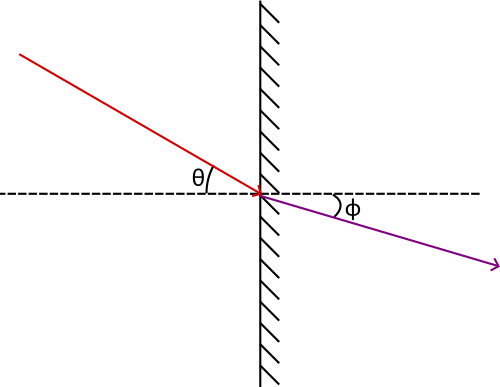
\includegraphics{../static/img/2026/refrection1}}

הפעם החלק המקוווקו לא מתאר מראה, אלא חומר כלשהו שהאור עובר דרכו, והשינוי
בזווית שהאור \textquotedblleft בוחר\textquotedblright{} בו הוא כדי
לאפטמז את המסלול. למה המסלול הוא לא קו ישר? ובכן, כי בחומר שמצד ימין
האור נע במהירות \textbf{שונה} מאשר בצד שמאל. זה כמובן מעלה את השאלה
- למה בעצם שאור ינוע במהירות שונה בתוך חומרים שונים? לזה יש תשובה
פיזיקלית יפה שאציג כאן בנפנוף ידיים פרוע: אור הוא גל \textbf{אלקטרומגנטי}.
הרעיון בגל כזה הוא שיש לנו שדה חשמלי שמשתנה לאורך זמן, והשינוי הזה
גורם להיווצרות שדה מגנטי שגם הוא משתנה לאורך זמן, והשינוי הזה גורם
להיווצרות שדה חשמלי... וכן הלאה. זה תופעה יפהפיה ממש כשמבינים אותה
וכמובן שלא אכנס כאן לפרטים שלה, אבל הפאנץ' הוא שבזכות החיזוק ההדדי
הזה, גל אלקטרומגנטי לא צריך \textbf{תווך} כדי להתקדם בו - להבדיל נאמר
מגלים בים, שצריכים מים, או גלי קול שצריכים אוויר. כשגל אלקטרומגנטי
פוגש חומר זה יכול רק להפריע, כי השדה האלקטרומגנטי \textbf{מעורר} את
החלקיקים בעלי המטען שבחומר, והם בתורם מייצרים גל אלקטרומגנטי משלהם
שמתערבב עם הגל המקורי ויוצר אפקט שאפשר לתאר בתור \textquotedblleft הגל
מאט\textquotedblright .

למרבה המזל, לא צריך להבין עד הסוף את המהומה הפיזיקלית הזו. השורה התחתונה
פשוטה מאוד: אם מהירות האור בריק, כששום דבר לא מפריע, היא \L{$c$},
אז כשהאור עובר בחומר מסוים המהירות תשנה אל \L{$v=\frac{c}{n}$} כאשר
\L{$n$} הוא קבוע \textbf{שמאפיין את החומר} שנקרא \textbf{מקדם השבירה}
של החומר. לחומרים שונים יש מקדמי שבירה שונים, ולכן בסיטואציה שלנו
נסמן את מקדם השבירה של החומר השמאלי ב-\L{$n_{1}$} ושל החומר הימני
ב-\L{$n_{2}$}. הקשר בין זווית הכניסה \L{$\theta$} וזווית היציאה
\L{$\phi$} יהיה תלוי באותם \L{$n_{1},n_{2}$}. אני יכול כמובן סתם
לתת את הנוסחה, אבל בואו נעשה משהו מעניין יותר ונשתמש בעיקרון פרמה
כדי למצוא אותה. אז כמו שעשינו קודם עם החזרה, בואו נשרטט דיאגרמה שבה
הקבועים הם הנקודות \L{$A,B$} של ההתחלה והסיום והמשתנה מספר לנו איפה
פוגעים בנקודה שבה עוברים מהתווך השמאלי לימני:

\L{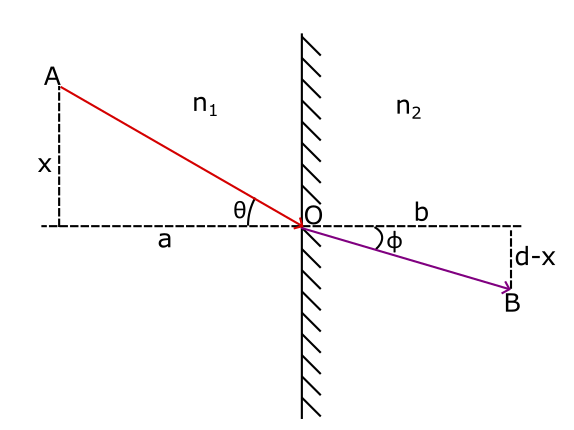
\includegraphics{../static/img/2026/refrection2}}

ועכשיו קורה פה קסם, כי אנחנו משחזרים כמעט לגמרי את החישוב שעשינו קודם.
האורך של הקו האדום הוא \L{$\sqrt{x^{2}+a^{2}}$} כמו קודם; והאורך
של הקו הסגול הוא \L{$\sqrt{\left(d-x\right)^{2}+b^{2}}$}. רק שעכשיו
אנחנו לא רוצים למנמז את סכום האורכים שלהם אלא את \textbf{הזמן} שלוקח
לעבור את המרחק הזה. אם יש לנו מרחק \L{$D$} כלשהו ואנחנו נעים במהירות
\L{$v$}, אז הזמן שנדרש לנו כדי לעבור את המרחק הוא \L{$\frac{D}{v}$}.
לכן במקרה שלנו, כשבצד שמאל נעים במהירות \L{$v_{1}$} ובצד ימין במהירות
\L{$v_{2}$}, אנחנו רוצים למנמז את הביטוי

\L{$T\left(x\right)=\frac{\sqrt{x^{2}+a^{2}}}{v_{1}}+\frac{\sqrt{\left(d-x\right)^{2}+b^{2}}}{v_{2}}$}

עכשיו אפשר להכניס את מקדמי השבירה לתמונה. כזכור, הרעיון במקדם שבירה
הוא שמתקיים \L{$v=\frac{c}{n}$}, כלומר \L{$\frac{1}{v}=\frac{n}{c}$}.
לכן אחרי הצבה בביטוי של \L{$T\left(x\right)$} נקבל

\L{$T\left(x\right)=\frac{n_{1}\sqrt{x^{2}+a^{2}}}{c}+\frac{n_{2}\sqrt{\left(d-x\right)^{2}+b^{2}}}{c}$}

החלוקה הזו ב-\L{$c$} לא משפיעה על הערך שמחזיר את נקודת המינימום,
אז מספיק לי למנמז את הפונקציה 

\L{$f\left(x\right)=n_{1}\sqrt{x^{2}+a^{2}}+n_{2}\sqrt{\left(d-x\right)^{2}+b^{2}}$}

עכשיו, אני \textbf{כבר יודע} איך גוזרים את השורשים המעצבנים הללו כי
עשיתי את זה קודם, והכפל ב-\L{$n_{1}$} ו-\L{$n_{2}$} לא משפיע כי
זה כפל בסקלר - פשוט כופלים בו בסוף. עכשיו, גזירה של \L{$\sqrt{x^{2}+a^{2}}$}
נתנה לנו את \L{$\frac{x}{\sqrt{x^{2}+a^{2}}}$} שבמקרה הקודם יצא שווה
לסינוס הזווית הרלוונטית - וגם עכשיו זה בדיוק מה שהוא יוצא! תעיפו מבט
במשולש שבאיור כדי לראות את זה. אנחנו מקבלים פה את \L{$\sin\theta$}.
באופן דומה גם הנגזרת של \L{$\sqrt{\left(d-x\right)^{2}+b^{2}}$} תיתן
לנו את \L{$\sin\phi$}, ולכן כמו שקודם קיבלנו את הנוסחה \L{$\sin\theta_{1}=\sin\theta_{2}$},
הפעם נקבל את הנוסחה

\L{$n_{1}\sin\theta=n_{2}\sin\phi$}

שלפעמים כותבים גם בתור

\L{$\frac{\sin\theta}{\sin\phi}=\frac{n_{2}}{n_{1}}$}

הנוסחה הזו נקראת \textbf{חוק סנל}. עכשיו אנחנו יודעים איך שבירה והחזרה
עובדות, ואפשר להגיע לאקשן - מה קורה לאור כשהוא פוגע בטיפה.

\section{הצד האפל של הקשת}

הנה העטיפה של האלבום \L{The Dark Side of the Moon} של פינק פלויד:

\L{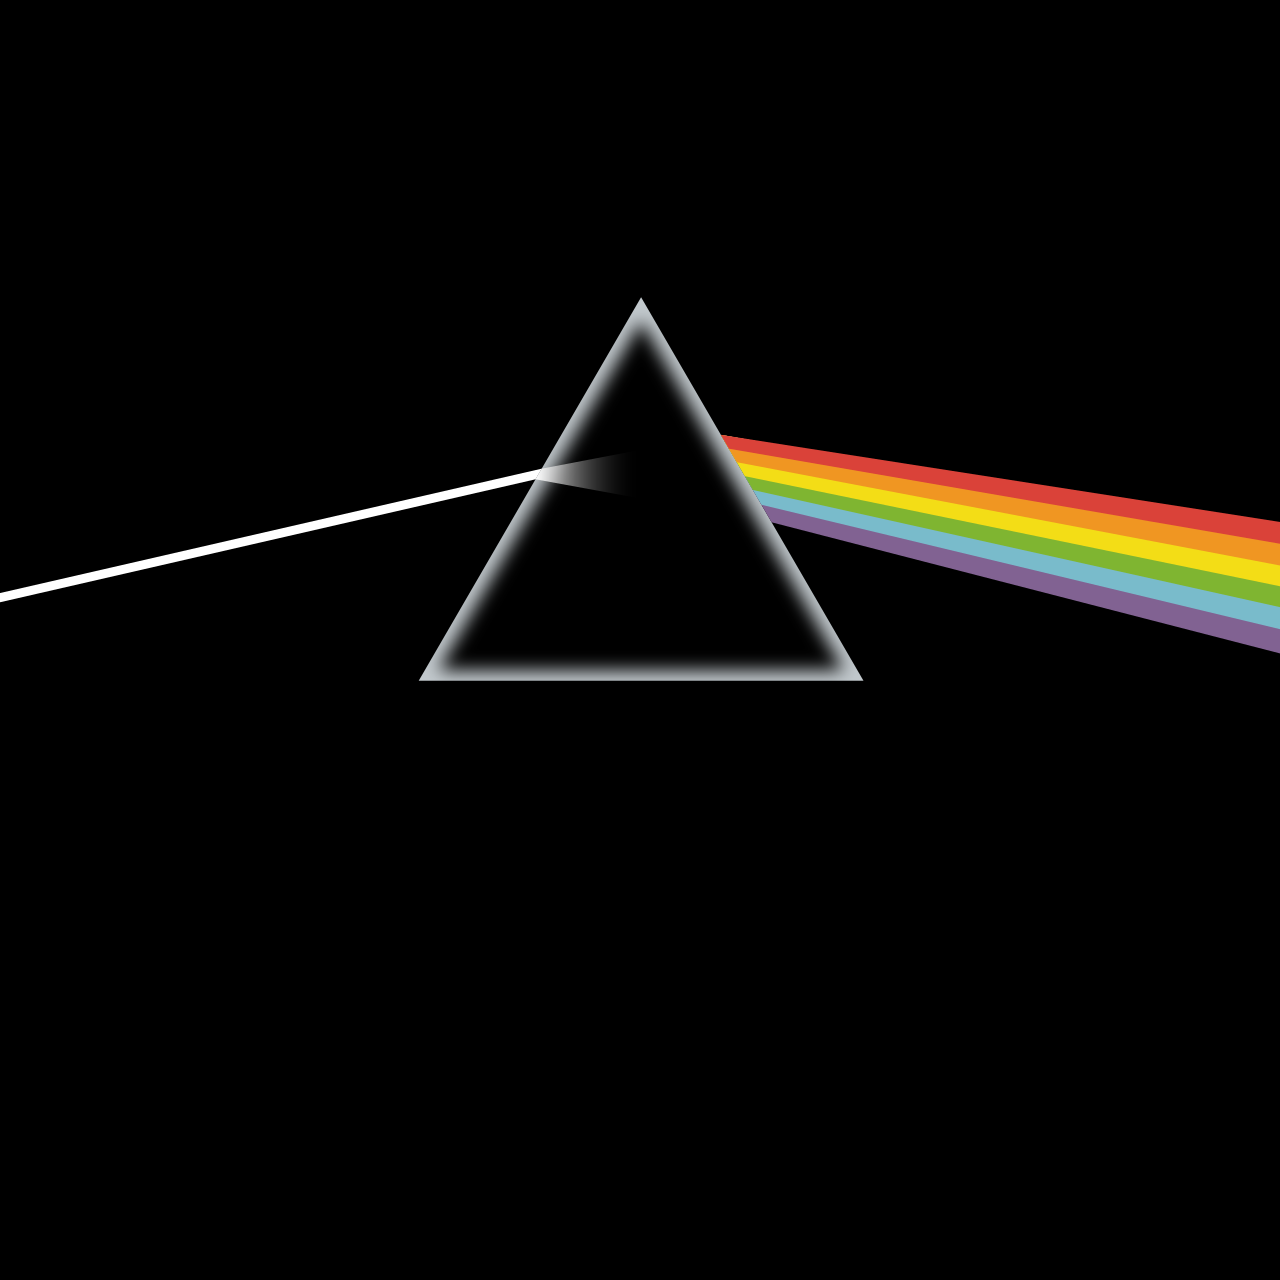
\includegraphics{../static/img/2026/the_dark_side_of_the_moon}}

מה שאנחנו רואים פה הוא דוגמא ל\textbf{פריזמה}, שהיא כלי שמפצל קרן
אור אחידה לצבעים שונים. בגלל הפופולריות של האלבום, זה כנראה הייצוג
המוכר ביותר לאנושות של פריזמה, וגם מה שאני זוכר עוד בתור ילד. זה ייצוג
טיפה חריג כי הוא לא מראה מה קורה \textquotedblleft בתוך\textquotedblright{}
הפריזמה, וגם מציג את האור המפוצל שיוצא החוצה עם שישה פסים במקום השבעה
המקובלים )הוא מאחד את סגול עם אינדיגו( - אבל כאמור, ההפרדה החדה הזו
לפסים שונים היא עניין תרבותי, לא פיזיקלי. הנה הדבר היותר קונבנציונלי
ש-\L{ChatGPT} מייצר כשמבקשים ממנו:

\L{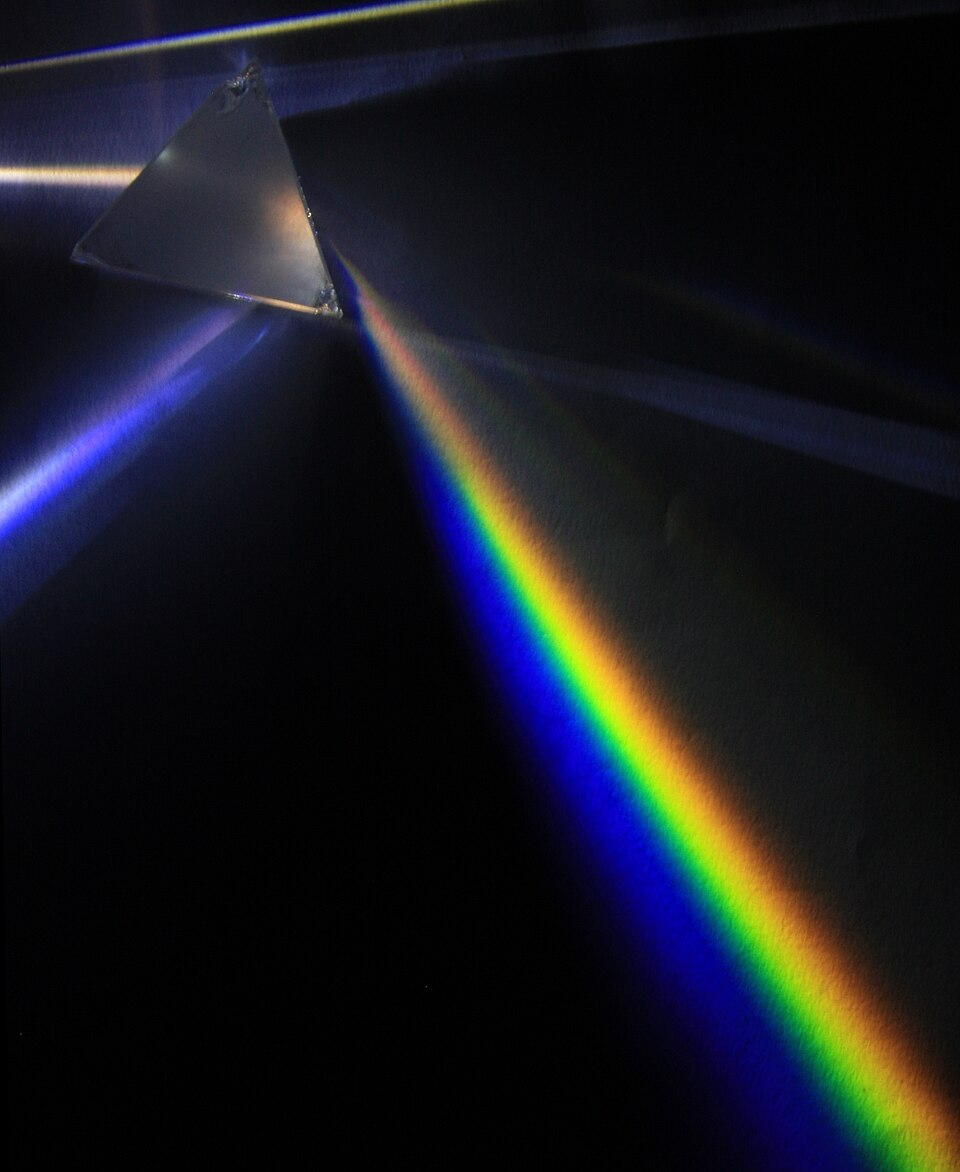
\includegraphics{../static/img/2026/prism}}

האיור הזה נותן תחושה קצת יותר ברורה של מה שקורה כאן: האור פוגע בפריזמה,
נשבר ומשנה כיוון \textbf{ומתפצל}, ואז פוגע בצד השני ועוד יותר נשבר
ומשנה כיוון )אבל כבר לא מתפצל שוב(. אנחנו כבר מבינים למה הוא נשבר
- זה חוק סנל בפעולה. אבל למה הוא מתפצל, מה שבפיזיקלית נקרא \textbf{נפיצה}?
בגלל דבר אחד שלא אמרתי עד כה: מקדם השבירה של חומר? המספר הזה שאומר
\textquotedblleft כמה החומר מאט את האור שעובר דרכו\textquotedblright ?
זה לא מספר אבסולוטי; זה מספר שתלוי \textbf{באורך הגל} של האור. לאותו
חומר בדיוק יש מקדמי שבירה שונים עבור אורכי גל שונים של אור. על פי
חוק סנל, זווית השבירה של האור תלויה במקדם השבירה של החומר, ולכן אורכי
גל שונים של אור יישברו בזוויות שונות - בדיוק כמו שרואים בדיאגרמה.
זה מה שגורם לקרן של \textquotedblleft אור לבן\textquotedblright{} )שהיא
בעצם קרן שמורכבת מקרני אור מכל הספקטרום של אורכי הגל של האור הנראה(
להתפצל בצורה כזו. עוד מעט נדבר על המתמטיקה של זה.

האיור של הפריזמה די נאמן למציאות. הנה תמונה מויקיפדיה:

\L{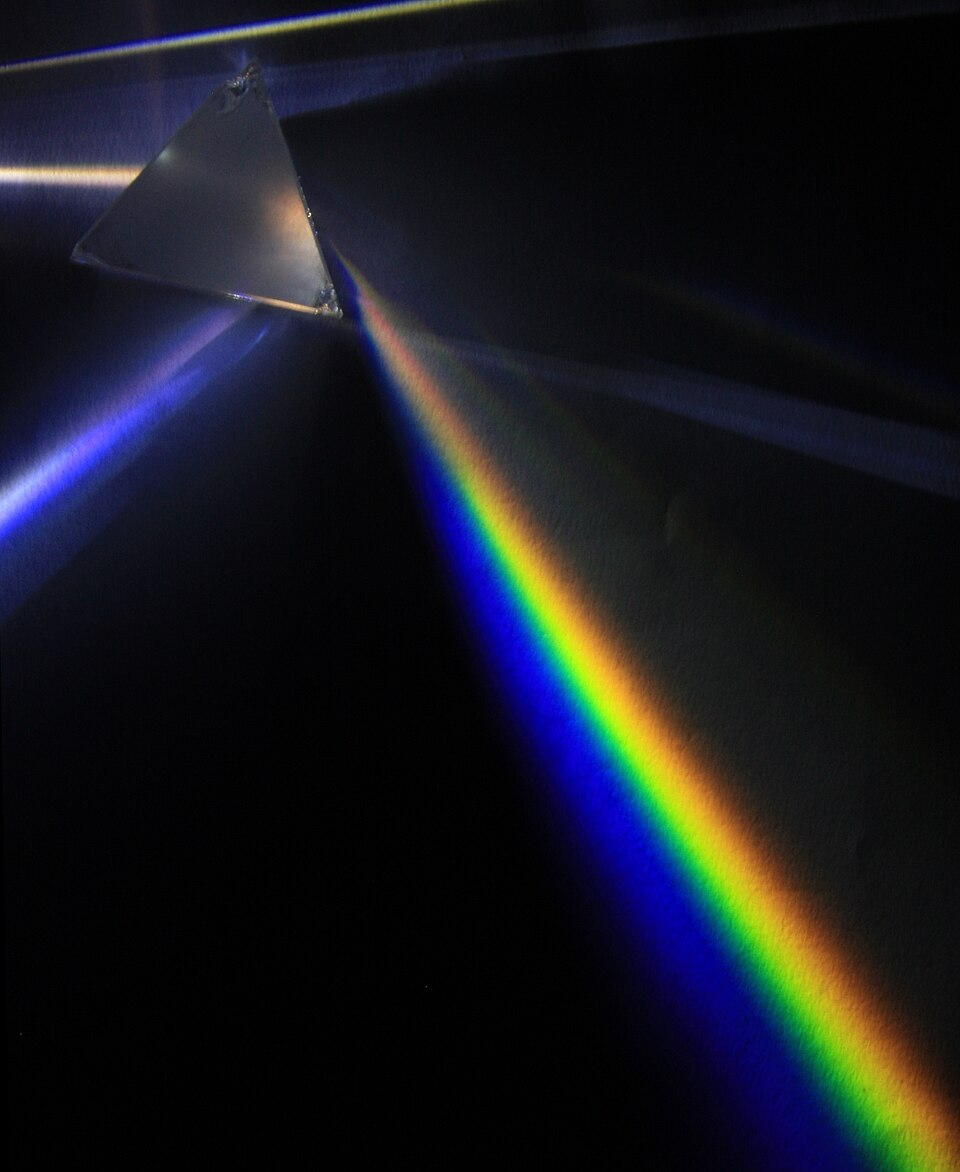
\includegraphics{../static/img/2026/prism}}

כמובן, הצבעים לא מופרדים פה בצורה ברורה כמו באיורים, אבל בהחלט אפשר
לראות את הקרן הנכנסת והקשת היוצאת. העניין הוא שכדי שנוכל לראות את
הסיטואציה הזו בפועל, צריכים להתקיים תנאי תאורה ספציפיים יחסית: החדר
צריך להיות חשוך, קרן האור שנכנסת לפריזמה צריכה להיות חזקה )ומורכבת
מצבעים מכל צבעי הקשת; לא כל מנורה עושה את זה(, וצריכים להיות חלקיקי
אבק באוויר שהאור יקפוץ מהם אל המצלמה אחרת לא נוכל לראות את הקשת \textquotedblleft באוויר\textquotedblright{}
כמו שקורה באיור הקלאסי - למרות שעדיין נוכל לראות את הקשת אם נשגר אותה
על קיר.

אם החדר יהיה מואר כולו אבל לא נשגר שום קרן על הפריזמה, לא נראה שום
קשת יפה למרות שאור עדיין עובר דרך הפריזמה ונשבר; זה בגלל שיגיע אור
מכל הכיוונים, יתפזר לכל הכיוונים, צבעים שונים ממקורות שונים יעלו אחד
על השני ובאופן כללי תהיה לנו מהומה. הנה עוד איור של \L{ChatGPT} שהוא
לא ממש מדויק אבל מבהיר את הכוונה:

\L{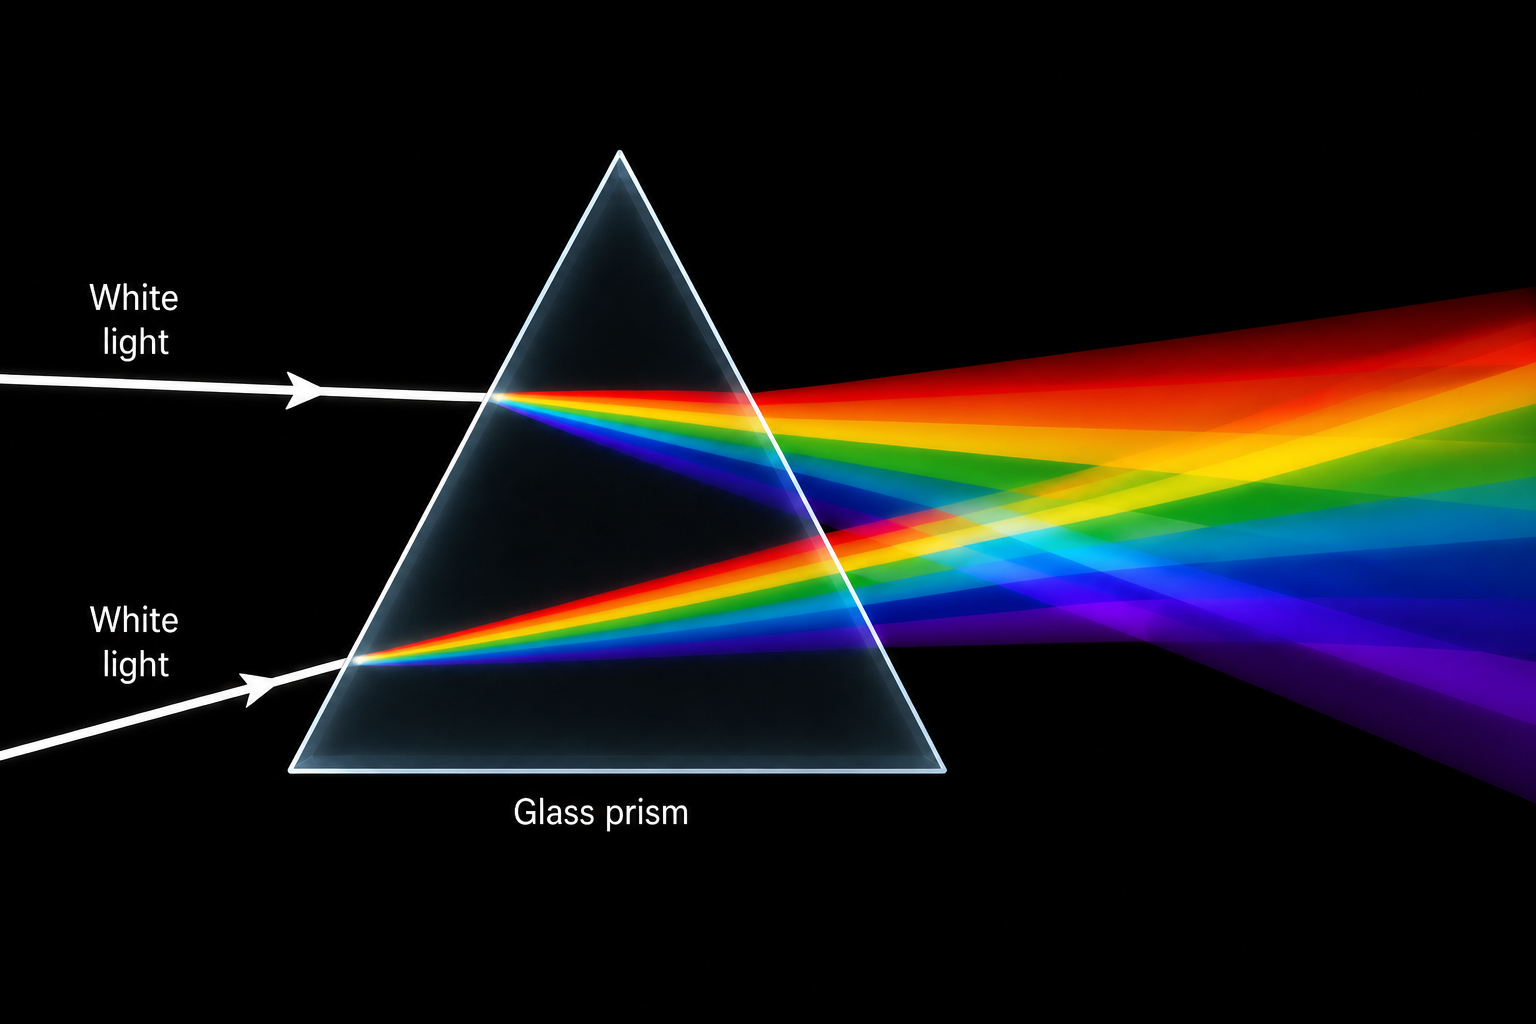
\includegraphics{../static/img/2026/prism2}}

השורה התחתונה היא שכדי שנראה קשת, לא מספיק לדבר על נפיצה; יש כאן שאלה
לא טריוויאלית של \textbf{ריכוז}. אנחנו צריכים שיהיה לנו איזור שיש
בו הרבה אור אדום ומעט מכל אור אחר, ואיזור עם הרבה אור סגול וכדומה.
\textbf{זה} הקסם שקורה בקשת וגורם לכך שנוכל לראות אותה ביום בהיר ולמרות
שהיא נוצרת מאור שמש שמורכב מהמון קרניים ולא קרן ממוקדת אחת )אבל, וזה
חשוב, המון קרניים \textbf{מקבילות}, כמו שאמרתי קודם(. איכשהו השילוב
הזה של שבירה והחזרה שמתרחש בתוך כל טיפה גורם ליצירה של איזור שבו האור
האדום מרוכז - אנחנו נראה שהריכוז הזה קשור איכשהו לזווית הפלאית {\beginL 42\endL}
){\beginL 42\endL}! התשובה לחיים, ליקום ובכלל!(. עבור צבעים אחרים
הריכוז יהיה קשור לזוויות קצת שונות, והריכוזים הללו בזוויות שונות הן
מה שגורם לקשת לעבוד.

אז בואו נראה מה קורה כשאור פוגע בטיפה ונסתכל קודם כל על אור \textbf{אדום},
אורך גל של {\beginL 750\endL} ננומטר. אני מצייר את קרן האור בתור קרן
אופקית, ומה שמעניין אותנו הוא מה \textbf{הגובה} של הקרן הזו ביחס לציר
האופקי שעובר דרך מרכז הטיפה. המקרה הפשוט ביותר הוא כשהגובה הזה הוא
אפס. זה נראה ככה:

\L{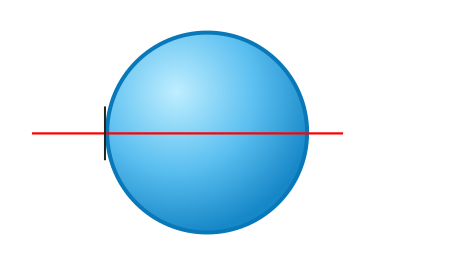
\includegraphics{../static/img/2026/rainbow_drop_stage3}}

אני מצייר קו שחור בנקודת הפגיעה שהוא המשיק לטיפה באותה נקודה - זה
ה\textquotedblright משטח\textquotedblright{} שבו הקרן פוגעת. במקרה
הזה, זווית הפגיעה של הקרן היא \L{$0^{\circ}$} כי הרי זווית הפגיעה
היא הזווית שהקרן יוצרת עם \textbf{האנך} למשטח, ובמקרה הזה הקרן עצמה
היא האנך למשטח. אם מכניסים את זה לחוק סנל:

\L{$n_{1}\sin\theta=n_{2}\sin\phi$}

אנחנו רואים שבכלל לא משנה מהם \L{$n_{1},n_{2}$}, באגף שמאל כתוב \L{$0$}
)כי סינוס של {\beginL 0\endL} הוא {\beginL 0\endL}( ולכן גם באגף ימין
חייבים שיהיה {\beginL 0\endL}, ומכיוון ש-\L{$n_{2}\ne0$} )כי מהירות
האור בתוך הטיפה היא לא {\beginL 0\endL}(, אז מקבלים שגם הזווית \L{$\phi$}
היא {\beginL 0\endL}. במילים אחרות, אין בכלל שבירה. \textbf{כן} יש
החזרה, בזווית של {\beginL 0\endL} מעלות - כלומר, חלק מהאור פוגע בטיפה
ומתחיל לזוז אופקית שמאלה במקום ימינה, וזה קורה פעמיים - פעם בכניסה
לטיפה ופעם ביציאה ממנה. אבל הקו של האור בתוך הטיפה נשאר ישר כל הזמן.

זה לא מעניין במיוחד. אז בואו נסתכל על מה שקורה כשאור נכנס יותר מגבוה:

\L{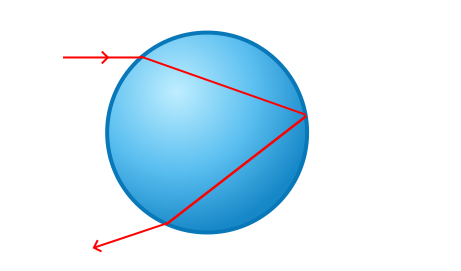
\includegraphics{../static/img/2026/rainbow_drop_stage4}}

כאן אפשר לראות את הסיפור המלא יותר: האור נשבר כשהוא נכנס לטיפה, פוגע
בקצה השני, קופץ חזרה ואז נשבר \textbf{שוב} כשהוא מגיע לגבול של הטיפה,
ויוצא משם בזווית כלשהי - הוא כבר לא אופקי כמו קודם. מה הזווית שבה
הוא פנה? ובכן, זה תלוי בשאלה כמה גבוה הוא היה - כלומר, באיזו זווית
הוא נכנס אל הטיפה )ככל שהוא יותר גבוה מעל קו האמצע, הזווית שבה הוא
נכנס תהיה קרובה יותר ל-\L{$90^{\circ}$}(. כדי לחשב את זה בצורה מסודרת,
בואו ניעזר בכך שהטיפה היא \textbf{עיגול} ואנחנו יודעים הרבה דברים
נחמדים על עיגולים. בפרט, בואו נמתח רדיוסים מנקודת האמצע של העיגול
אל שלוש הנקודות על השפה שלו שבהן מתרחש האקשן - שתי השבירות וההחזרה.
ככה זה ייראה:

\L{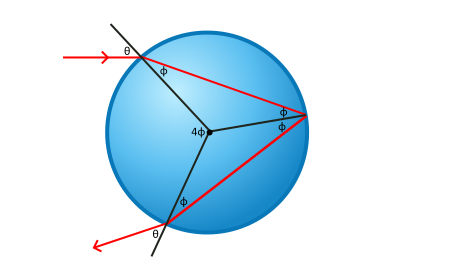
\includegraphics{../static/img/2026/rainbow_drop_stage5}}

אוקיי, מה קורה פה? ראשית, בואו נזכור משהו בסיסי מגאומטריה: רדיוס תמיד
מאונך למשיק בנקודת ההשקה - כלומר, אם אני מאריך את הרדיוס קצת מעבר
לנקודה על שפת העיגול, אני מקבל את \textbf{הנורמל למשטח} שביחס אליו
אנחנו מודדים זווית עבור שבירה והחזרה. אני מסמן ב-\L{$\theta$} את
זווית הפגיעה למעלה, וב-\L{$\phi$} את מה שמתקבל ממנה אחרי השבירה.
חוק סנל כבר לימד אותנו שמתקיים \L{$n_{1}\sin\theta=n_{2}\sin\phi$}.
כדי לפשט אני יכול לסמן \L{$n=\frac{n_{2}}{n_{1}}$} ולקבל \L{$\sin\theta=n\sin\phi$}.

השלב הבא הוא מה שקורה בנקודה שבה יש החזרה. שימו לב ששני הרדיוסים שמתחתי
לנקודת השבירה העליונה ונקודת ההחזרה יוצרים \textbf{משולש שווה שוקיים}
)כי כל הרדיוסים מאותו אורך( ובמשולש שווה שוקיים זווית הבסיס שוות,
ולכן זווית הפגיעה בקצה הימני היא \L{$\phi$} ולכן גם זווית ההחזרה
היא \L{$\phi$} ולכן מקבלים גם למטה \L{$\phi$} מאותו נימוק של משולש
שווה שוקיים, ולכן חוק סנל מספר לנו שהאור הולך לצאת החוצה באותה זווית
\L{$\theta$} שבה הוא נכנס - אבל זו זווית \textbf{ביחס לנורמל} באותה
נקודה, זה עדיין לא מספר לנו כמה בעצם האור התעקם ביחס לקו האופקי המקורי.

כאן נכנס לתמונה עניין ה-\L{$4\phi$} שכתוב במרכז. מה שקורה פה הוא
עוד משפט מגאומטריה אוקלידית בפעולה: \textquotedblleft גודלה של זווית
היקפית, הנשענת על אותה קשת שעליה נשענת זווית מרכזית, שווה לחצי גודלה
של הזווית המרכזית.\textquotedblright{} כמו שאומרים בויקיפדיה העברית
כרגע. הזווית ההיקפית המדוברת היא הזווית שבצד ימין, שמורכבת משני ה-\L{$\phi$}-ים.
היא נשענת על הקשת השמאלית שמחברת את נקודת הכניסה והיציאה של האור.
על אותה קשת נשענת גם הזווית שנוצרת משני הרדיוסים שמגיעים לנקודות הכניסה
והיציאה, ונפגשים שניהם במרכז המעגל. \textquotedblleft זווית מרכזית\textquotedblright{}
היא בדיוק דבר כזה - זווית שנוצרת משני רדיוסים. הזווית ההיקפית היא
מגודל \L{$2\phi$} ולכן הזווית המרכזית היא מגודל \L{$4\phi$}.

עכשיו, הזווית המרכזית יותר מתחילה כשהיא \L{$\theta$} מעלות \textbf{יותר}
מהקרן שנכנסת, ומסיימת כשהיא \L{$\theta$} מעלות \textbf{יותר} מהקרן
שיוצאת. אז אם אנחנו רוצים לדעת את הזווית היחסית בין הקרן שנכנסת לקרן
שיוצאת, אנחנו צריכים לחסר ולקבל \L{$4\phi-2\theta$}. את הביטוי הזה
אפשר לייצג גם בתור פונקציה של זווית הפגיעה \L{$\theta$} בלבד; אני
אקח את הנוסחה \L{$\sin\theta=n\sin\phi$} של חוק סנל ואפעיל \L{$\sin^{-1}$}
)\textquotedblleft ארקסינוס\textquotedblright ( על שני האגפים, כך
שיתקבל \L{$\phi=\sin^{-1}\left(\frac{\sin\theta}{n}\right)$}. את
זה אני אציב בנוסחה שקיבלתי לפני רגע, ואקבל:

\L{$\alpha\left(\theta\right)=4\sin^{-1}\left(\frac{\sin\theta}{n}\right)-2\theta$}

את המשחק הזה אפשר לשחק עם הרבה קרניים ולבדוק מה זווית היציאה בכל אחד
מהמקרים. אם עושים את זה, קורה משהו מעניין שאפשר לראות פה:

\L{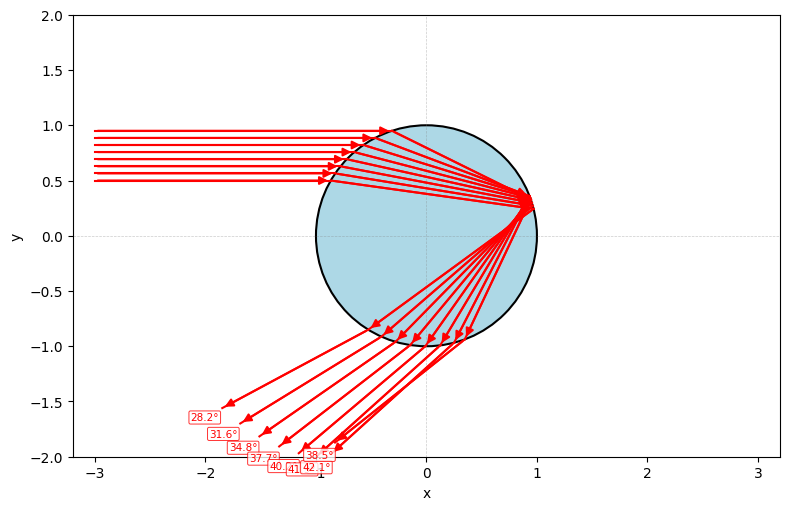
\includegraphics{../static/img/2026/rainbow_drop_matplotlib1}}

מה שקורה הוא שכשאנחנו מעלים עוד ועוד את הקרן שפוגעת בטיפה - כלומר,
מגדילים עוד ועוד את \L{$\theta$}, אז זווית היציאה לא ממשיכה לגדול
עוד ועוד - מתישהו היא מתחילה ליפול חזרה. במילים מתמטיות, לפונקציה
\L{$\alpha\left(\theta\right)$} יש \textbf{מקסימום מקומי}. התוצאה
היא שנוצר \textbf{ריכוז} של אור אדום בסביבות הזווית של המקסימום המקומי
הזה. כמו שאפשר לראות מהאיור, יוצא הרבה אור אדום בהרבה זוויות שונות,
אבל יש טווח זוויות ספציפי שבו הוא \textbf{מרוכז} וזה בערך \L{$42^{\circ}$}.
פחות או יותר {\beginL 10\endL} אחוזים מהקרניים יתרכזו באיזור הזה בזמן
שהיתר יכסו די באחידות את יתר טווח הזוויות.

הריכוז הזה הוא \textbf{הסיבה המרכזית} שבגללה קשת בענן קיימת, וזה מה
שלא הצלחתי לתפוס עד שלא התחלתי להתעמק בנושא )לא שזה סוד גדול; בכל
הסבר על קשת פתאום יופיע המספר הקסום \L{$42^{\circ}$}, אבל לפעמים
בלי להכריח את עצמך להתעמק אתה לא קולט עד הסוף מה המשמעות שלו(.

מה קורה עם סגול? ובכן, אותו הדבר רק \textbf{עם זווית שונה}:

\L{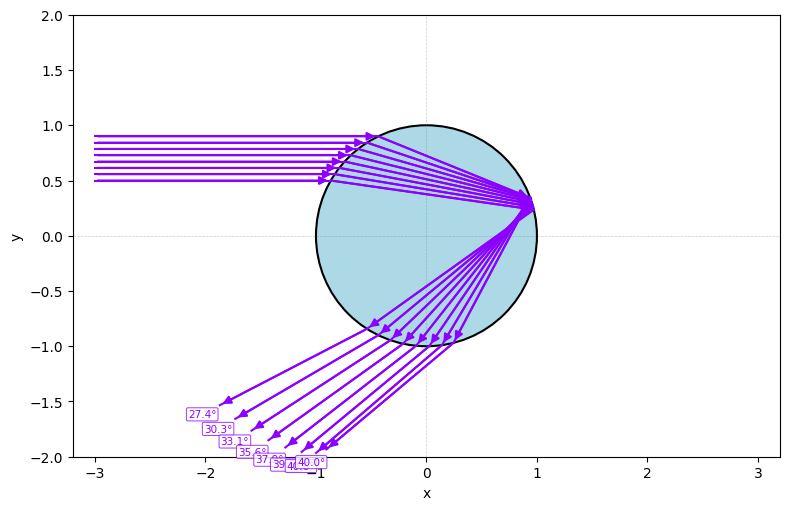
\includegraphics{../static/img/2026/rainbow_drop_matplotlib2}}

כאן הזווית היא בסביבות \L{$40^{\circ}$}. ומכיוון שאדום וסגול הם קצוות
הסקלה, זה אומר שכל המהומה שמתרחשת בקשת היא בגלל טווח הזויות הקטן הזה,
\L{$40^{\circ}-42^{\circ}$}. אבל עדיין צריך להסביר איך זה בדיוק קורה
- הרי אמרתי שקשת היא תהליך תלת-שלבי:
\begin{enumerate}
\item השמש פולטת קרני אור שמגיעות לכדור הארץ.
\item קרני האור הללו עוברות דרך איזור באוויר שמלא בטיפות מים.
\item התוצאה של המפגש הזה של קרני האור והמים מגיעה אל העיניים שלנו.
\end{enumerate}
עכשיו אנחנו מבינים את {\beginL 2\endL} )אחרי שבתקווה הבנו קודם את
{\beginL 1\endL}( אבל אני עדיין צריך לדבר קצת על {\beginL 3\endL}.

לפני שנעשה את זה, בואו נעשה קצת \textbf{מתמטיקה}. יש לי את הפונקציה
\L{$\alpha\left(\theta\right)=4\sin^{-1}\left(\frac{\sin\theta}{n}\right)-2\theta$};
אני רוצה למצוא את \L{$\theta$} שעבורו נקבל את נקודת המקסימום של הפונקציה.
המקסימום הזה יהיה כמובן תלוי בקבוע \L{$n$} שבתורו תלוי בתכונות של
האוויר, של המים ושל אורך הגל של האור שאני מסתכל עליו כרגע.

אז מה עושים? חשבון דיפרנציאלי ואינטגרלי בסיסי. גוזרים. ראשית, אני
ממש לא זוכר איך גוזרים ארקסינוס, אז אני מסתכל בדף נוסחאות:

\L{$\left(\sin^{-1}\left(z\right)\right)^{\prime}=\frac{1}{\sqrt{1-z^{2}}}$}

בשלב הזה כבר ברור שזה הולך להיות כואב, אבל לא להתייאש - \textbf{נגזרות
זה קל} כי לא צריך להיות יותר מדי יצירתיים. עכשיו, איך אני גוזר משהו
כמו \L{$\sin^{-1}\left(\frac{\sin\theta}{n}\right)$} שבו אין משתנה
חמוד בפנים? בעזרת כלל השרשת:

\L{$\left(f\left(g\left(\theta\right)\right)\right)^{\prime}=f^{\prime}\left(g\left(\theta\right)\right)g^{\prime}\left(\theta\right)$}

כאשר \L{$f=\sin^{-1}$} זה אומר שנקבל

\L{$\frac{g^{\prime}\left(\theta\right)}{\sqrt{1-g^{2}\left(\theta\right)}}$}

וזה עבור \L{$g\left(\theta\right)=\frac{\sin\theta}{n}$} בעלת הנגזרת
\L{$g^{\prime}\left(\theta\right)=\frac{\cos\theta}{n}$}. עכשיו,
הייתי רוצה לפשט את הזוועה של \L{$\sqrt{1-g^{2}\left(\theta\right)}$}
שבמכנה, אז הנה טריק: כזכור, \L{$\sin\phi=\frac{\sin\theta}{n}$},
אז \L{$g\left(\theta\right)=\sin\phi$}, ולכן \L{$\sqrt{1-g^{2}\left(\theta\right)}=\sqrt{1-\sin^{2}\phi}=\cos\phi$},
תוך שימוש בזהות הטריגונומטרית הסטנדרטית \L{$\sin^{2}\phi+\cos^{2}\phi=1$}.
לכן קיבלנו

\L{$\alpha^{\prime}\left(\theta\right)=\frac{4}{n}\frac{\cos\theta}{\cos\phi}-2$}

וזה... ביטוי די חמוד? אנחנו רוצים להשוות אותו ל-{\beginL 0\endL},
כך שנקבל

\L{$\frac{4}{n}\frac{\cos\theta}{\cos\phi}-2=0$}

שהופך אל

\L{$\frac{2}{n}\frac{\cos\theta}{\cos\phi}=1$}

או במילים אחרות

\L{$2\cos\theta=n\cos\phi$}

בואו נצרף לזה את הקשר המקורי בין הזוויות:

\L{$\sin\theta=n\sin\phi$}

אני רוצה להיפטר איכשהו מ-\L{$\phi$} לחלוטין. טריק אחד לעשות את זה
הוא להשתמש בזהות \L{$\sin^{2}\phi+\cos^{2}\phi=1$} שכבר ראינו. בשביל
לעשות את זה, צריך להעלות את שתי המשוואות בריבוע, ולחבר:

\L{$4\cos^{2}\theta+\sin^{2}\theta=n^{2}\left(\cos^{2}\phi+\sin^{2}\phi\right)=n^{2}$}

עכשיו יש לנו גם קוסינוס וגם סינוס ביחד, אבל כשהם בריבוע יש לנו קשר
נחמד בינם כמו שכבר ראינו: \L{$\cos^{2}\theta=1-\sin^{2}\theta$},
אז קיבלנו

\L{$4-3\sin^{2}\theta=n^{2}$}

ולכן

\L{$\sin^{2}\theta=\frac{4-n^{2}}{3}$}

כלומר

\L{$\theta=\sin^{-1}\left(\sqrt{\frac{4-n^{2}}{3}}\right)$}

עכשיו אפשר להציב ערכים קונקרטיים. דיברתי על אור אדום של {\beginL 750\endL}
ננומטר? אני לא מכיר נוסחה פשוטה שבעזרת אורך הגל מחזירה את אינדקס השבירה
של האוויר והמים ביחס לאור הזה, אבל אלו ערכים שכמובן אפשר לחשב אמפירית
בניסוי ולכן אפשר סתם למצוא אותם באינטרנט ולמלמל \textquotedblleft פיזיקה...\textquotedblright .
מתברר שיש ממש אתרים שמתעסקים בזה! למשל \L{https://refractiveindex.info/}!
הוא אמר לי שעבור {\beginL 750\endL} ננומטר, אינדקס השבירה של מים הוא
\L{$n_{2}=1.3295$} ואינדקס השבירה של אוויר... אה... לא מצאתי שם אוויר...
אבל באוויר יש בעיקר חנקן! ועבורו הוא נתן \L{$n_{1}=1.00029659$} שזה
די דומה לערך המעוגל של \L{$1.0003$} שבו תמיד משתמשים!

...

אני לא טוב בכל העסק הזה של פיזיקה, מה.

מכל מקום, עכשיו אפשר לחשב 

\L{$n=\frac{n_{2}}{n_{1}}=\frac{1.3295}{1.00029659}\approx1.329106$}

וזה נותן \L{$\theta\approx59.637$} ו-\L{$\phi\approx40.480$} ולכן
\L{$4\phi-2\theta\approx42.648$} שזה... בערך... זווית ה-\L{$42^{\circ}$}
המדוברת! זה באמת עובד!

טוב, מספיק חישובים להיום או לאי פעם.

\section{איפה כל זה פוגש אותנו}

כל מה שראינו עד עכשיו על קשת דיבר על מה שקורה ברמת \textbf{הטיפה הבודדת}
כשאור השמש מגיע אליה. ראינו איך פגיעה כזו גורמת לחלק מהאור לעבור דרך
הטיפה )וזה לא מעניין( ולחלק מהאור \textbf{לחזור}, אבל לא רק בתור השתקפות
\textquotedblleft סתם\textquotedblright{} למרות שבהחלט חלק מהאור חוזר
ככה. ספציפית, בזווית מאוד מסויימת, סביבות \L{$42^{\circ}$} יהיה ריכוז
גדול יחסית של אור \textbf{אדום}, ובזווית קצת פחות גדולה של אור \textbf{כתום}
וכן הלאה עד שבסביבות \L{$40.5^{\circ}$} יהיה ריכוז של אור \textbf{סגול}.
את האפקט הזה הדגים לי \L{ChatGPT} עם האיור הבא:

\L{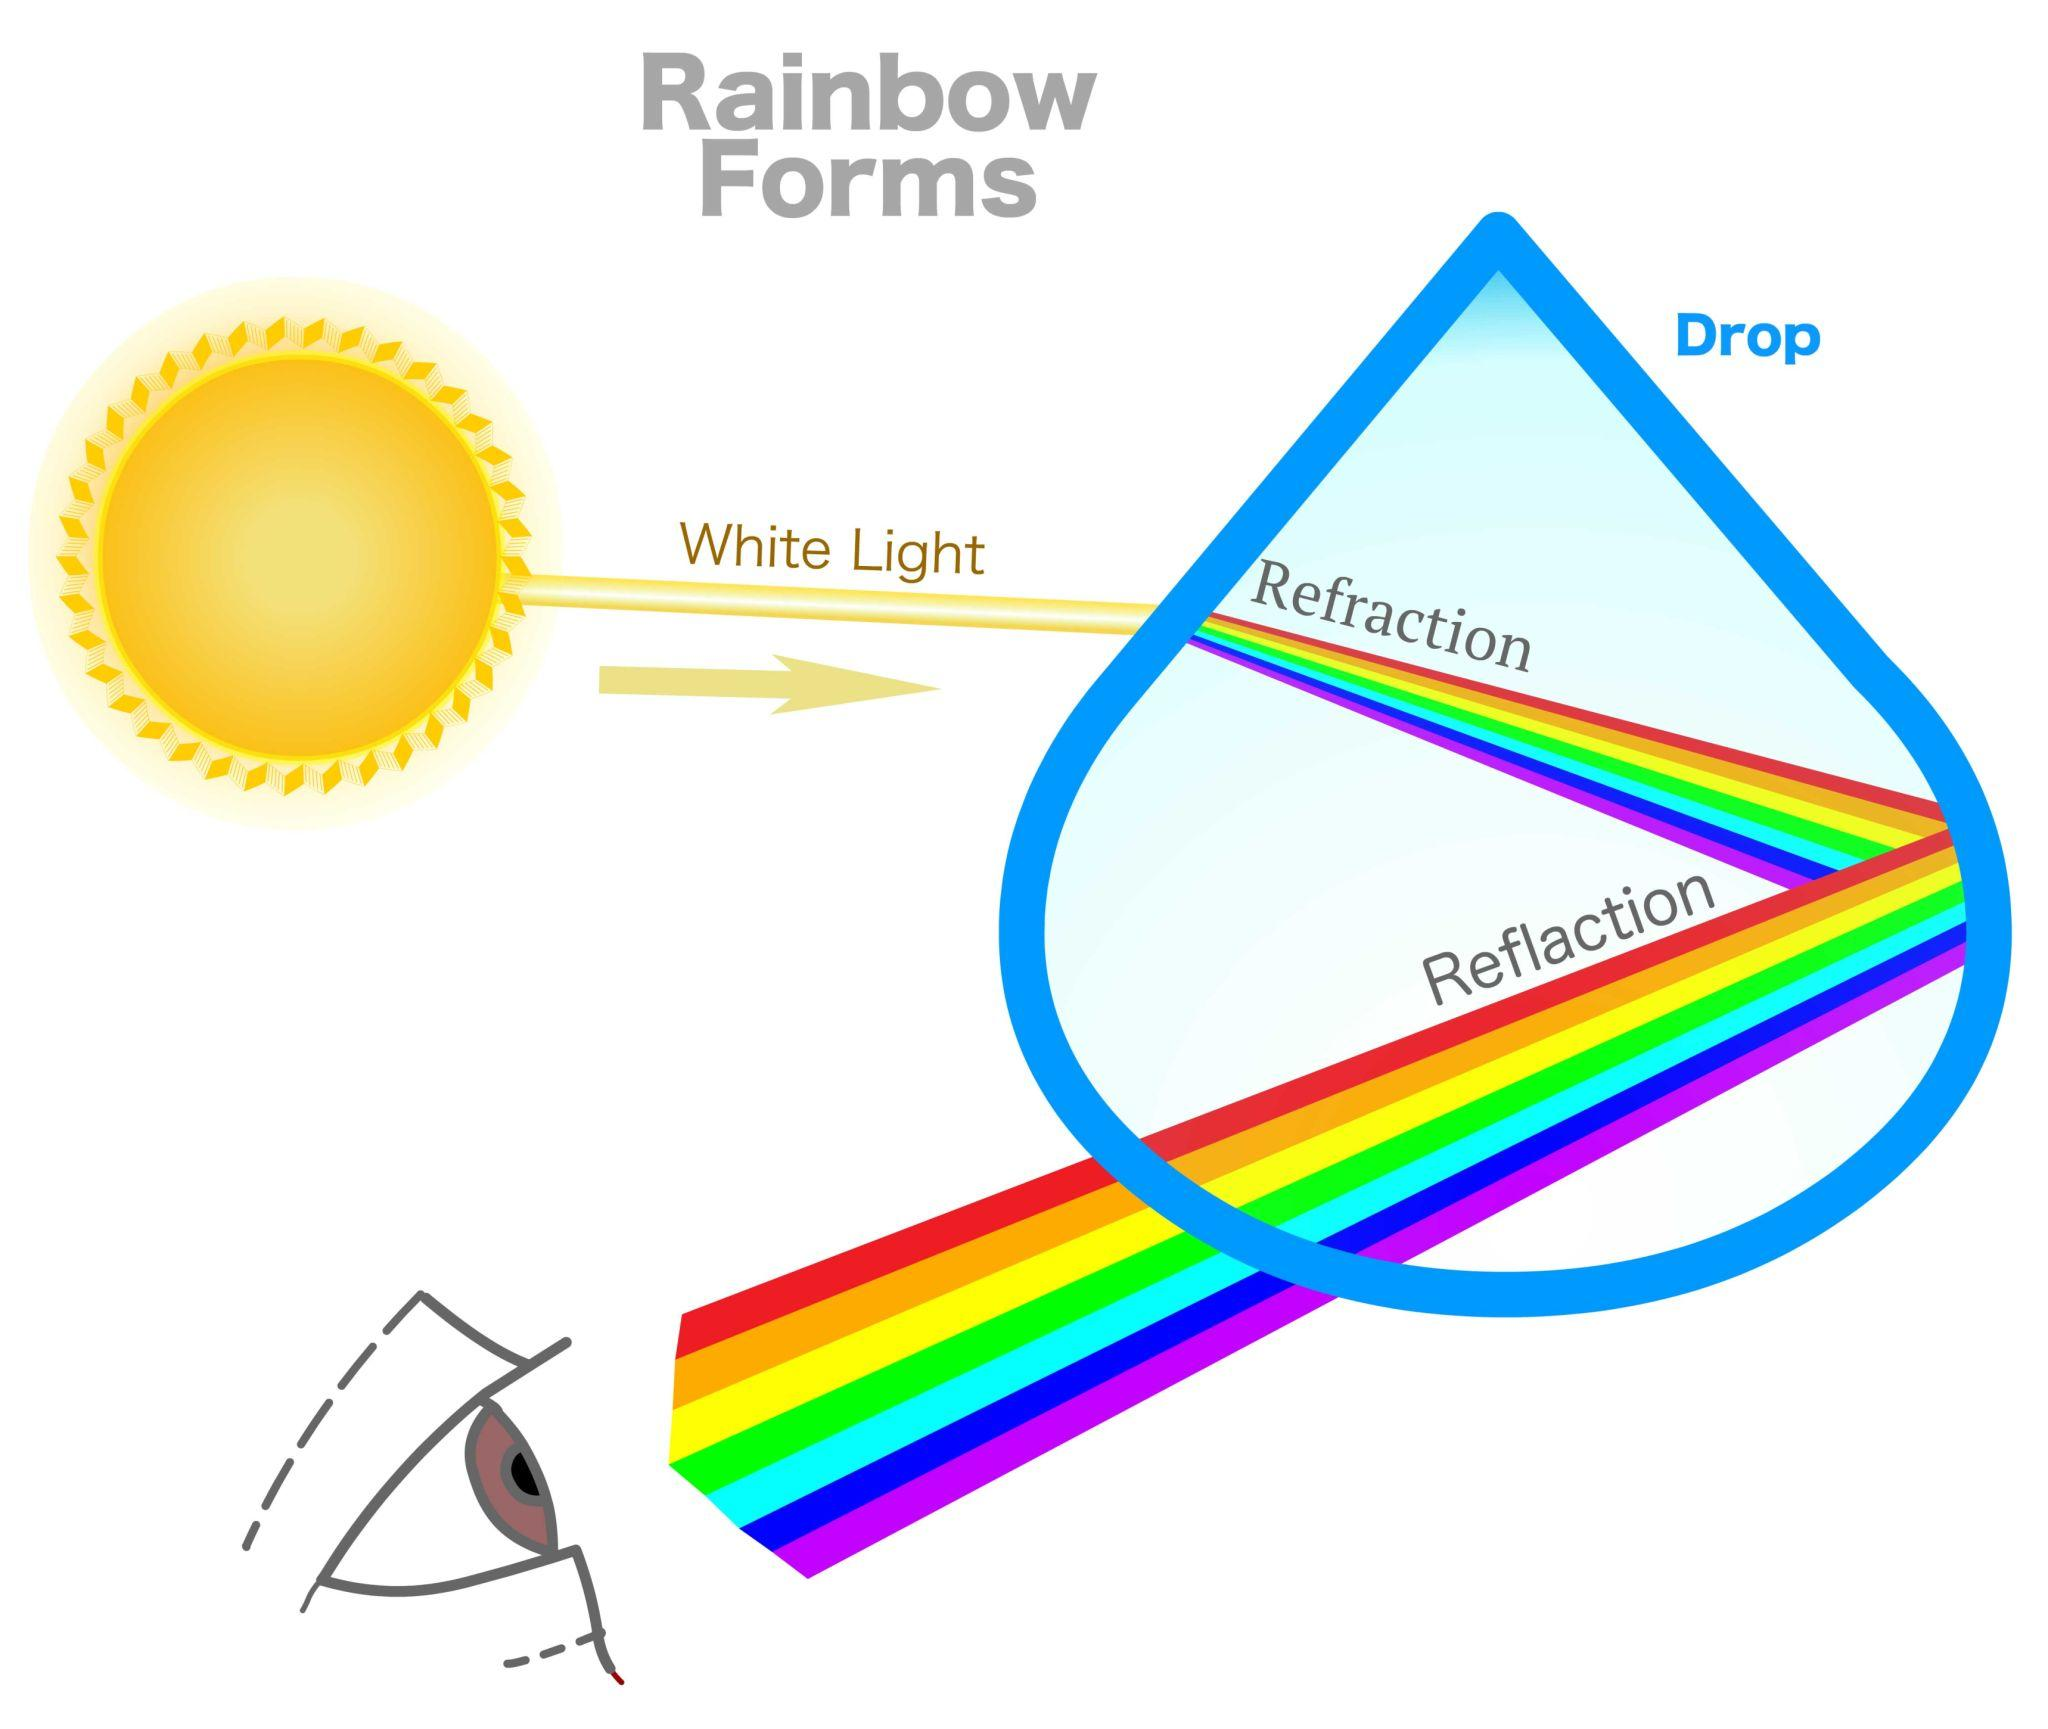
\includegraphics{../static/img/2026/rainbow1}}

כבר אמרתי שאני אוהב את האיור הזה כי הוא \textbf{שגוי לגמרי} בכל הנוגע
לשלב של האור שמגיע אל העין; ושגוי לגמרי באותה הצורה שהטעתה אותי תמיד
לגבי קשת בענן, ובאמת אפשר לראות כמו בהרבה דיאגרמות. הבעיה באיור היא
שנראה שהאור פוגע בטיפה אחת ספציפית, מתפצל, \textbf{וכל הקרניים} מגיעות
לעיניים שלי. כלומר, זה יוצר את הרושם השגוי שכשאני רואה קשת בענן אני
רואה אפקט \textbf{נקודתי}. התפיסה השגויה שלי הלכה צעד אחד קדימה וחשבה
משום מה שנקודת ה\textquotedblright מרכז\textquotedblright{} של הקשת
שבה אין צבעים בכלל )הרי קשת היא מעגל שחצי ממנו מוסתר - גם על זה עוד
נדבר פה - ולכן יש לה מרכז( - זו הנקודה שבה בעצם אור השמש פוגע בטיפות
וקופץ חזרה מהן ומגיע לעיניים שלי. זה \textbf{לא מה שקורה}, אבל כמה
שהיה קל לי להתפתות ולחשוב שזה קורה. לזכותי ייאמר שזה לא לגמרי מופרך
לחשוב ככה. הנה צילום מסך מהסרטון \L{What They (Probably) Don't Teach
You About Rainbows At School} של ערוץ היוטיוב \L{Veritasium} שמציג
בצורה מעולה את כל הנושא:

\L{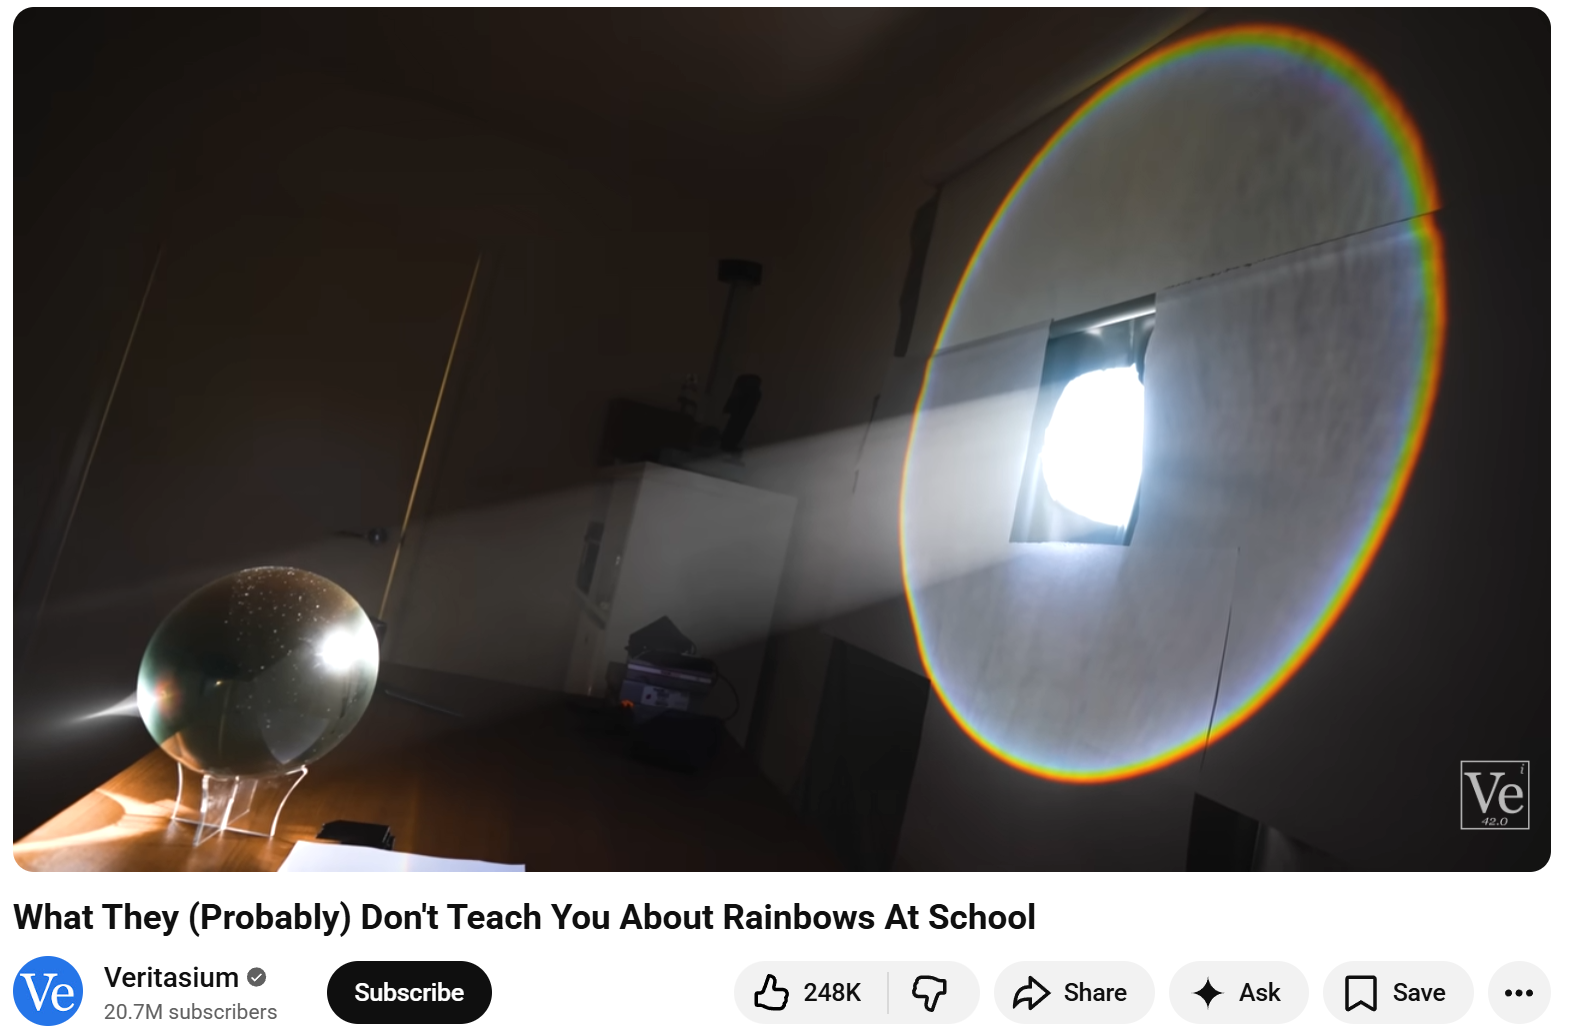
\includegraphics{../static/img/2026/veritaserum_rainbow}}

מה שאנחנו רואים פה הוא הדגמה של מה קורה ברמת הטיפה הבודדת, שאותה מחליף
כאן כדור זכוכית שאור השמש מאיר עליו ישירות ואז הוא מקרין על הקיר את
ה\textquotedblright קשת\textquotedblright{} שנוצרת מכך. כאן הצבעים
שאנחנו רואים באמת מגיעים כולם מאותו מקור נקודתי וזה נראה כאילו הכדור
נמצא במרכז העיגול, בחלק ש\textquotedblright אין בו קשת\textquotedblright .
זו הייתה האינטואיציה הכללית שלי.

אבל כשרואים משהו מרוחק מאיתנו שמתפרש על פני מרחק גדול, לא כל הקרניים
מגיעות מאותו מקום - קרניים ממקומות שונים שנעות בזוויות שונות מגיעות
אל האירוע הנקודתי שהוא העיניים שלנו. אפילו בצילום המסך מהסרטון - מה
שאנחנו רואים בפועל הוא את התוצאה של אור שפגע בקיר \textbf{במקומות
שונים} ואז קפץ מהקיר אל עבר המצלמה.

כשאנחנו רואים קשת בענן, אנחנו רואים אור שמגיע אלינו מהמון טיפות שונות
במרחב שאור השמש הישיר מגיע אליהן. עבור רובן, האור שהן מחזירות מהשמש
\textbf{וגם מגיע אלינו} הוא כזה שיוצא בזווית שבה לא מתקבלים צבעים
יפים ואנחנו לא רואים כלום וזה למרות שאותן טיפות בדיוק \textbf{כן מוציאות}
אור בצבעים יפים, פשוט לא לכיוון שלנו; אבל עבור חלקן, אנחנו נמצאים
בדיוק בזווית הנכונה כדי שאותן טיפות יחזירו אלינו, נאמר, אדום.

בואו נראה איך זה קורה. לדעתי הכי נוח לדמיין את הגשם בתור מין \textquotedblleft מסך\textquotedblright{}
שבו אור השמש פוגע, למרות שמסך הוא משטח דו ממדי ובמציאות טיפות המים
נמצאות בתוך איזור תלת ממדי ואור השמש בהחלט יכול לפגוע בכולן - זה אומר
שיש הרבה טיפות ב\textquotedblright עומק\textquotedblright{} של המסך
שמחזירות אלינו אור אדום ולא רק אלו שנמצאות על \textquotedblleft פני
השטח\textquotedblright . אין עם זה בעיה כי כל האורות האדומים הללו
נעים ביחד ומחזקים אלו את אלו. אז הנה איור שבו אני מצייר כמה \textquotedblleft מסכים\textquotedblright{}
בזה אחר זה:

\L{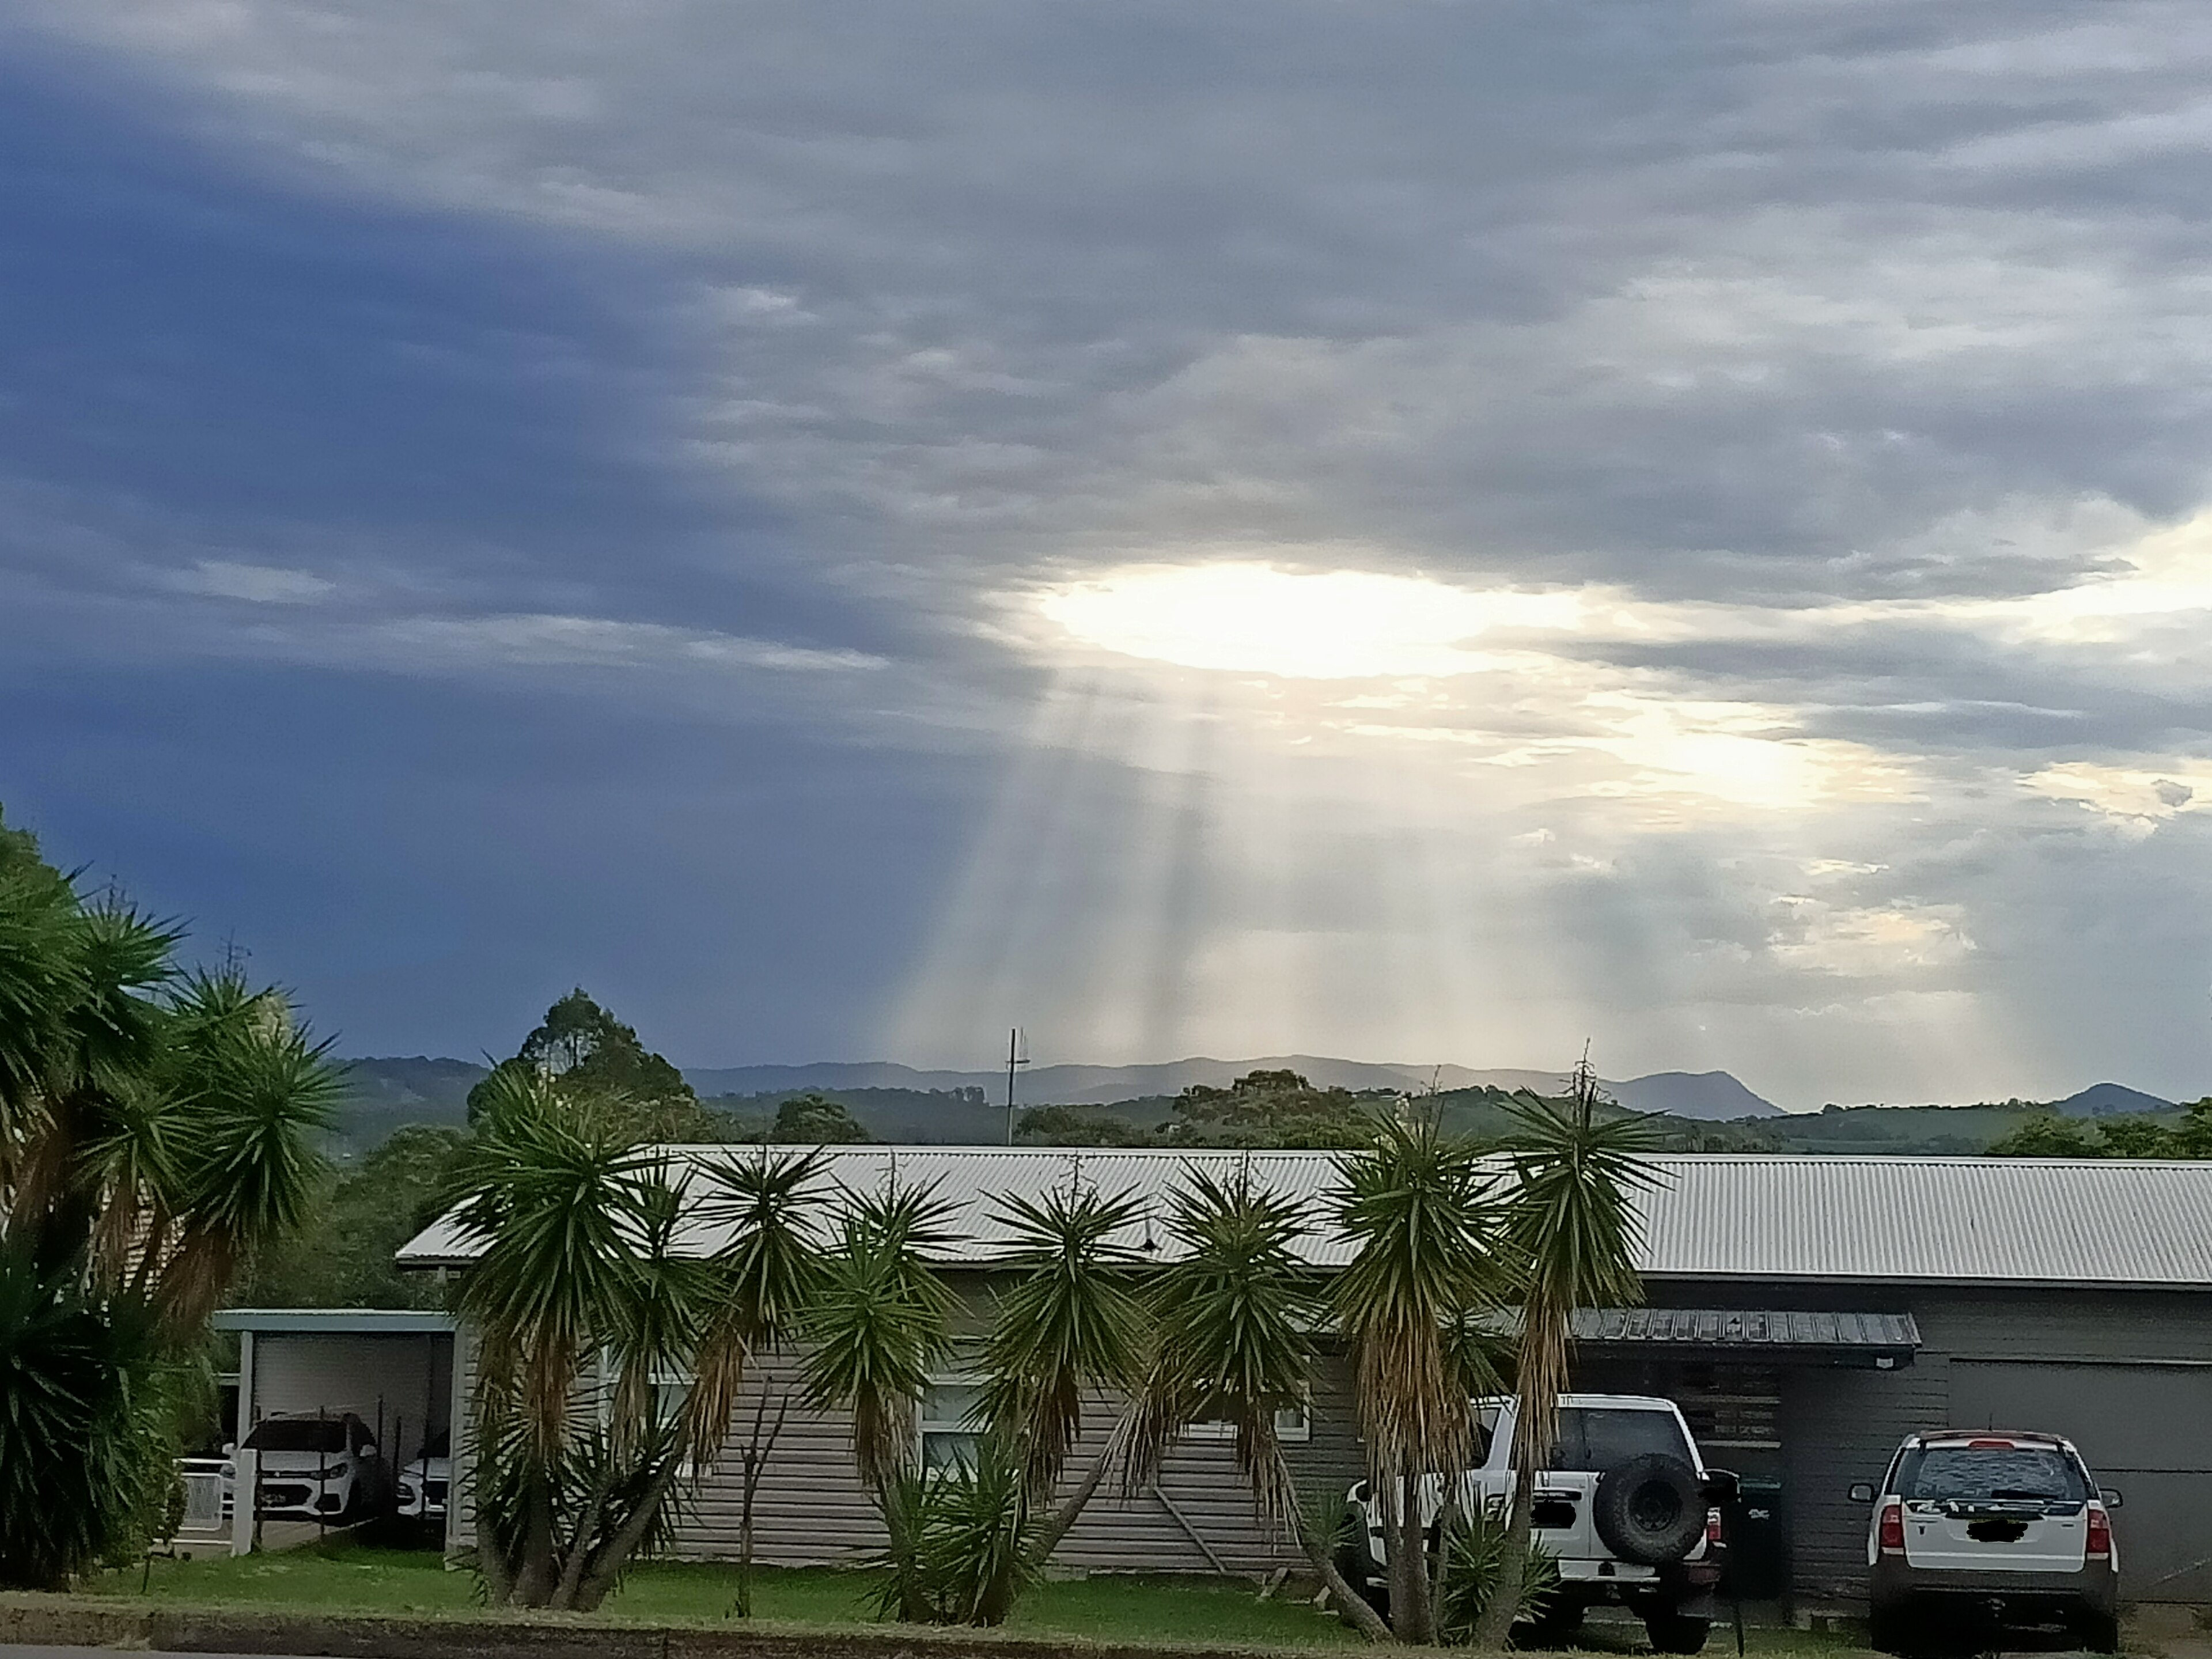
\includegraphics{../static/img/2026/rainbow5}}

ההפרה בין האדום והסגול באיור הזה גרועה מאוד כי אני מתעקש להשתמש בזוויות
\L{$42^{\circ}$} ו-\L{$40.5^{\circ}$} שטרחתי לחשב קודם. אין הצדקה
אמיתית לפדנטיות הזו חוץ מהטראומה שלי מאינספור שנים של איורים לא מדויקים
שגרמו לי לעבוד על עצמי. באיור הזה, הזווית שבה האור מגיע מהשמש היא
נמוכה יחסית - \L{$15^{\circ}$}. האור פוגע בטיפות, חוזר לכל הכיוונים
עבור כולן, אבל יש קו אחד מאוד ספציפי בזווית \L{$42^{\circ}$} )ביחס
לכיוון של אור השמש( שיוצא מהעין שלנו ומגיע אל הטיפות - ורק טיפות שנמצאות
על הקו הזה ישלחו את האור האדום המרוכז שיוצא מהן ישר אלינו.

כמובן, זה לא באמת נכון שיש רק \textbf{קו אחד} כזה. יש כזה כי התמונה
היא דו ממדית. הקו הולך רק \textquotedblleft ימינה\textquotedblright .
אבל בפועל, יש גם קווים בזווית {\beginL 42\endL} שהולכים \textquotedblleft ימינה
ולתוך התמונה\textquotedblright{} או \textquotedblleft ימינה ומחוץ לתמונה\textquotedblright .
אפשר לחשוב על זה ככה: אתם עומדים ומביטים בקשת הישר לפנים - אפשר לדמיין
שיש קו שיוצא מכם בדיוק בכיוון שאליו אתם מסתכלים. יש רק קו אדום אחד
של אור שמגיע אלינו בדיוק מהכיוון של הקו הזה. אבל אם נזוז אפילו \textbf{טיפה}
הצידה, כבר יהיה קו אדום \textbf{אחר} שמגיע אלינו. בגלל שזזנו טיפה
הצידה, הוא כבר לא יוכל להגיע מנקודה באותה גובה - משהו צריך להתקזז,
אז הנקודה שלו תהיה קצת יותר גבוהה או נמוכה. מה שנקבל הוא צורה של \textbf{חרוט},
קונוס, שלא היה לי כוח לצייר בעצמי כי זה תלת ממד ואני נוראי בזה, אז
ביקשתי מ-\L{ChatGPT} שיתעלל בהתאם בתמונה הקודמת ויוציא פלט שאני מזהיר
מראש שהוא \textbf{מאוד לא מדויק}:

\L{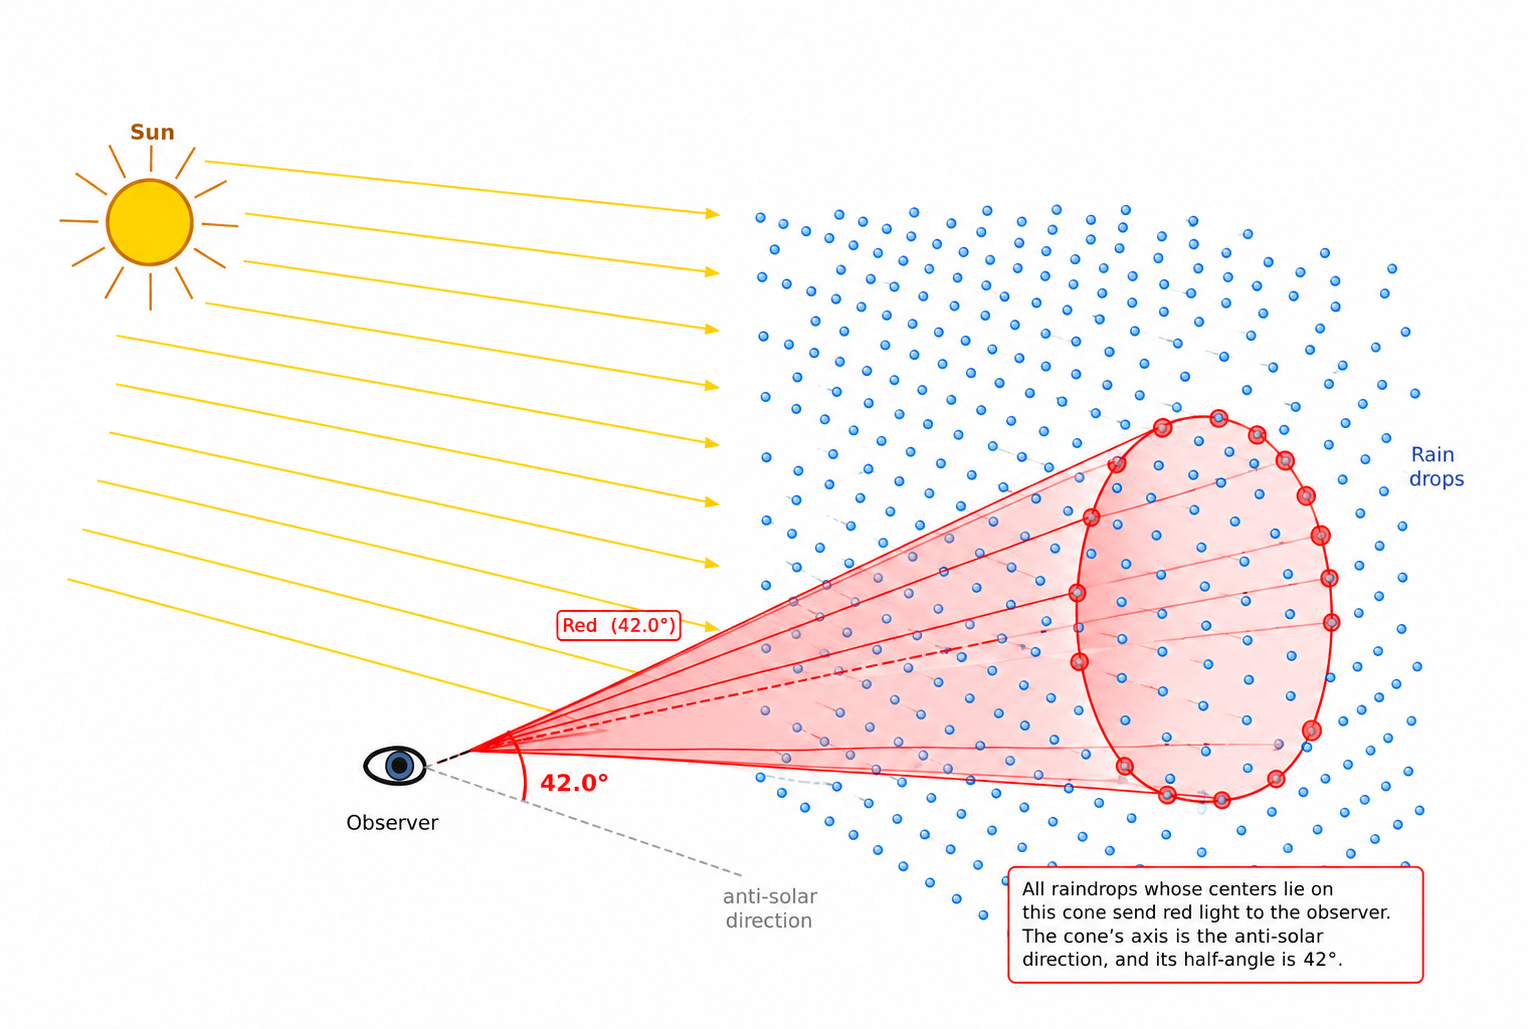
\includegraphics{../static/img/2026/rainbow6}}

מעניין להשוות את זה לתמונה מהסרטון של \L{Veritasium} - שם הייתה לנו
\textquotedblleft טיפה\textquotedblright{} נקודתית שהוציאה חרוט של
אור; כאן אנחנו עושים סוג של ההפך, החרוט מתרכז בעין שלנו, אבל האורות
מגיעים משלל טיפות שונות ומשונות.

אלא שגם הפעם \L{ChatGPT} טועה ומטעה באיור שלו, כי הוא מצייר \textbf{מעגל
שלם} כאילו גם החלק התחתון שלו הוא גבוה מהעין - אבל במקרה הזה, איך
ייתכן שגם האור מהחלק העליון וגם מהחלק התחתון מגיעים באותה זווית? לא,
החלק התחתון צריך להיות \textbf{מתחת} לגובה העין, והנה הבעיה - בדרך
כלל כשאנחנו רואים קשת, \textbf{אין} טיפות מים באוויר שהן \textquotedblleft מתחת
לגובה העין\textquotedblright{} במרחק. במרחק מה שאנחנו רואים הוא לרוב
שטוח או אפילו נהיה גבוה יותר. אבל אם אנחנו על הר גבוה ומסתכלים למטה
בהחלט נוכל לראות עוד מהקשת ואולי גם את העיגול כולו, וגם כשאנחנו מעופפים
באוויר - בין אם במטוס ובין אם בצניחה חופשית למשל. הנה עוד תמונה יפה
מויקיפדיה האנגלית:

\L{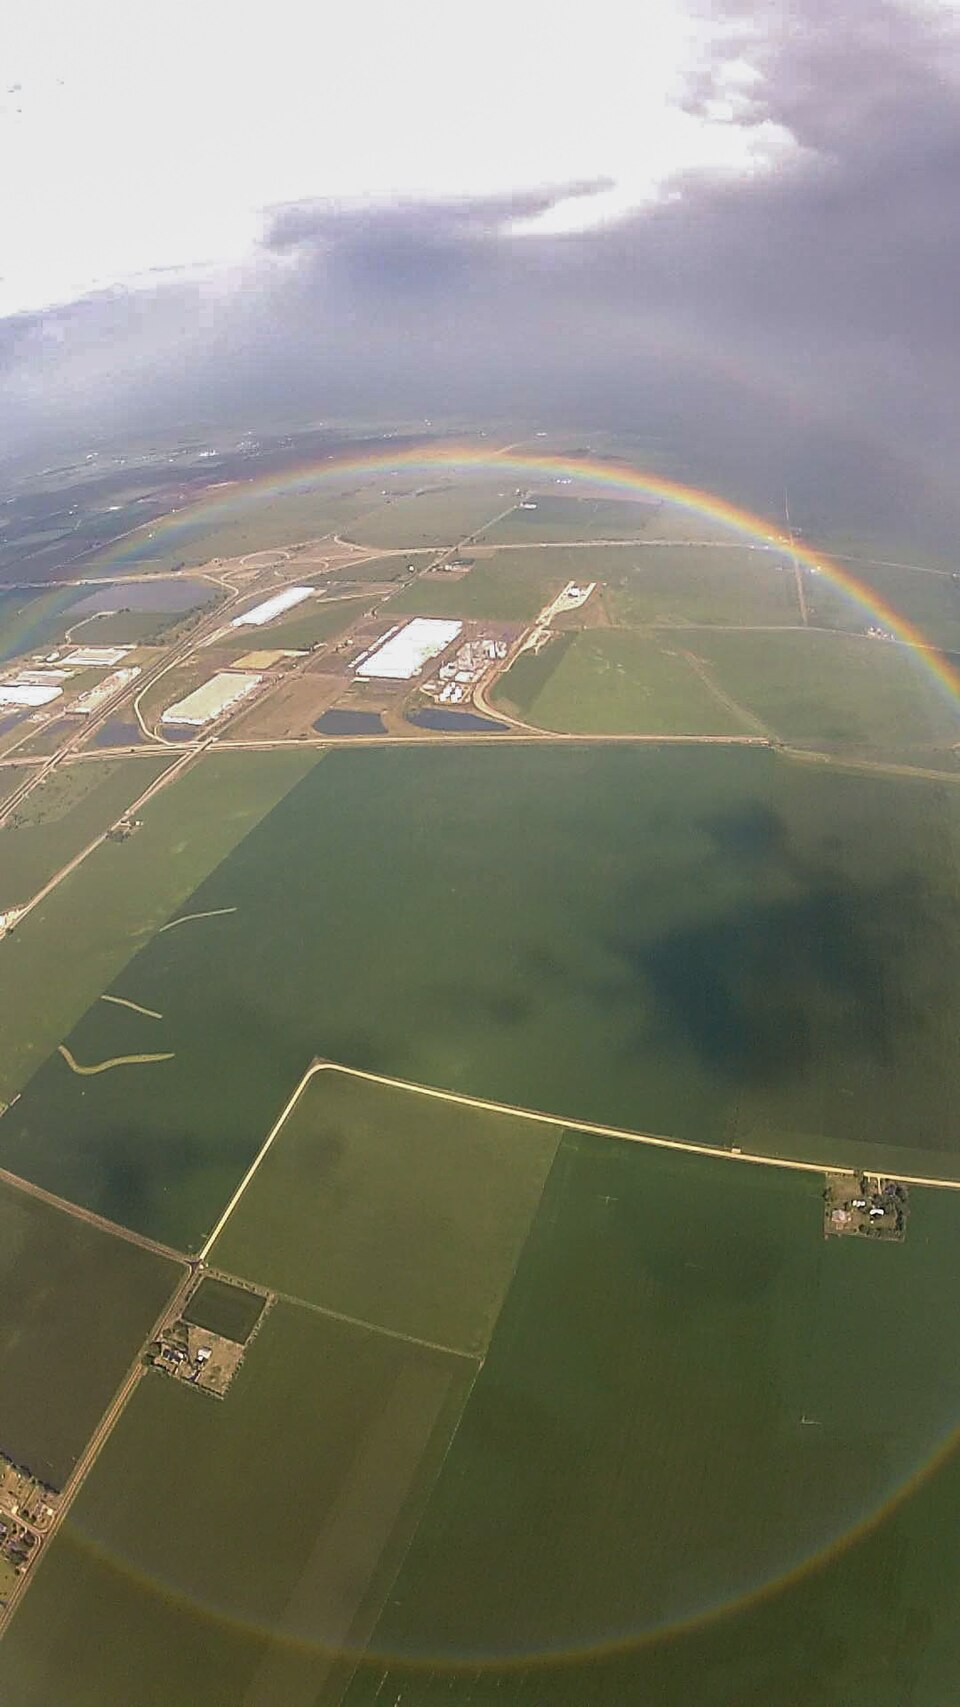
\includegraphics{../static/img/2026/Circular_rainbow}}

אבל רגע! בתמונה הזו חוץ מהקשת עצמה רואים... עוד קשת...? חלשה יותר?
עם סדר צבעים הפוך? כן, זו תופעה שנקראת \textbf{קשת כפולה} והיא די
נפוצה. ברשותכם אני אוותר על הניתוח המתמטי שלה להפעם, אבל היא נגרמת
מאותם עקרונות - רק שהפעם האור שאנחנו רואים הוא כזה שמשתקף \textbf{פעמיים}
בתוך הטיפה ולא רק פעם אחת )ולכן הקשת חלשה יותר - בכל פעם שאור משתקף
חלק ממנו הולך לאיבוד כשהוא נשבר החוצה(.

הקטע הזה שאנחנו לא רואים את כל הקשת רוב הזמן מן הסתם רק הולך ומחמיר
ככל שחושבים על זה. הבעיה היא לא רק עם דברים שמתחת לאופק. הבעיה היא
עם כל איזור בשמיים שאין בו טיפות - ולכן אנחנו רואים לפעמים קשת חלקית
בלבד, פשוט כי אין מה שיחזיר את האור באיזורים הרלוונטיים הנוספים בשמיים.
ובעיה חמורה לא פחות היא שהשמש \textbf{זזה} בשמיים וככל שהיא עולה כך
הזווית של הקרניים גדולה יותר. תראו מה קורה לאיור המסכן שלי כשאני מגדיל
את הזווית ל-{\beginL 30\endL} מעלות:

\L{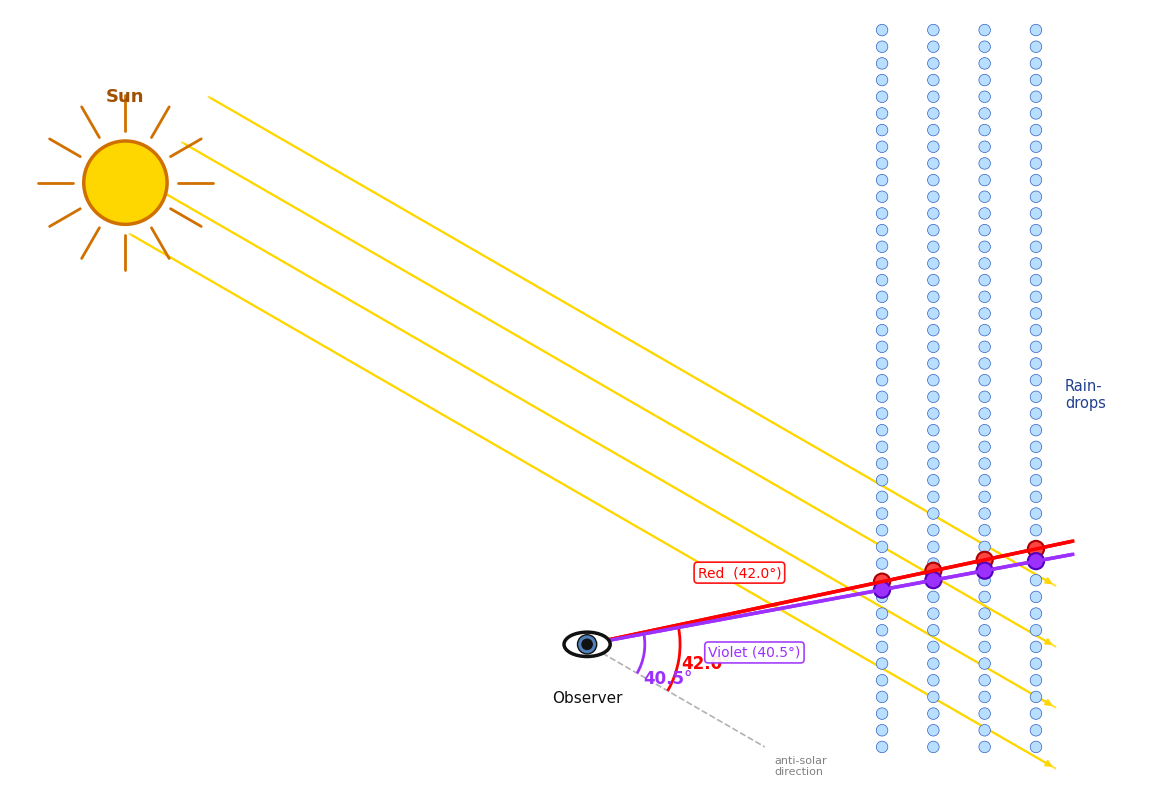
\includegraphics{../static/img/2026/rainbow7}}

כשאני אומר \textquotedblleft זווית של {\beginL 42\endL} מעלות\textquotedblright ,
הכוונה לזווית בין הכיוון של קרני השמש וכיוון הקרן האדומה שמגיעה לעין
שלי. ככל שקרני השמש מגדילות את הזווית שלהן ביחס לציר האופקי, הקרנים
האדומות צריכות \textbf{להקטין} את הזווית שלהן ביחס לציר האופקי - הן
נעשות יותר ויותר שטוחות, עד שנגיע למצב שבו השמש שולחת קרניים בזווית
של \L{$42^{\circ}$} ואז הקרניים יהפכו לאופקיות - משלב זה ואילך הקשת
תהיה נמוכה מדי מכדי שנראה אותה )אלא אם, שוב, אנחנו על הר או במטוס
או בצניחה חופשית או משהו(. זו הסיבה שבגללה בדרך כלל רואים קשתות בבוקר
או אחר הצהריים, כשהשמש נמוכה יותר בשמיים.

עוד נקודה אחת שתמיד בלבלה אותי היא ההנחה השגויה שכשיש קשת, \textquotedblleft כולנו\textquotedblright{}
רואים את אותה הקשת. אני רואה קשת יפה וממהר לצלם אותה ואז האינטרנט
מתמלא בצילומים של אותה קשת מזוויות שונות! אבל, כמובן, זו לא אותה קשת.
אנחנו מצלמים את אותו איזור בשמיים שיש בו כרגע טיפות מים והשמש מאירה
עליו באופן ישיר - אבל הצבעים שאני רואה מגיעים מטיפות שונות מאשר הצבעים
שרואה מי שצילם תמונה דומה במרחק {\beginL 100\endL} מטרים ממני. זו
הסיבה האמיתית שבגללה אי אפשר \textquotedblleft להגיע אל קצה הקשת\textquotedblright{}
- לא בגלל שהקצה הזה הוא סתם אור ולא משהו גשמי )כי אור הוא משהו גשמי!
ואנחנו רואים אור שקפץ חזרה מטיפת מים, זה מאוד גשמי!( אלא בגלל שכל
אחד מאיתנו רואה את הקצה הזה במקום שונה.

אז... נראה לי שזהו! אני הצלחתי לפייס את עצמי סוף סוף בכל הנוגע לקשתות.
אני כבר לא מרגיש שמישהו מרמה אותי, אני חושב שהבנתי בערך למה זה קורה,
ואני יודע שבפעם הבאה שבה יורד גשם ואז פתאום יוצאת שמש המקום שאני צריך
לפנות אליו כדי לחפש קשת הוא כזה שבו השמש היא \textbf{מאחורי}, ורצוי
כשאני משקיף מגובה של הר, ושזה יהיה בבוקר או אחר הצהריים, ואם הצלחתי
לראות קשת אז לא לוותר על לבדוק אם אפשר לראות קשת כפולה. מי אמר שמתמטיקה
זה לא פרקטי?
\end{document}
